\chapter{尿色异常}

正常新鲜排出的尿液呈淡黄色而透明。尿色主要由尿色素(urochrome),尿胆素(urobilin)和尿红素(uroerythrin)所致。当尿液放置后可形成微量絮状沉淀,这是由于少量上皮细胞、核蛋白和黏蛋白所构成。尿的颜色改变和颜色深浅受尿量的多少、尿渗透压和尿pH的影响。尿量多时,尿色浅而透明;尿量少、尿液浓缩时,尿色深而黄。酸性尿色深,碱性尿色浅。尿色还受内源性含色素的食物、药物、体内代谢产物、内源性血红蛋白、肌红蛋白、脓尿、乳糜尿的影响。新鲜尿液放置后发生混浊可能由于:①尿酸盐沉淀:加热或加碱可溶解。②磷酸盐和碳酸盐沉淀:加酸后可溶解,碳酸盐加酸后可产生气泡(二氧化碳)而逸出。

通常地,通过详细询问饮食和服药史,并结合常规尿检可初步了解色素来源。

\section{【临床意义较大的尿色异常】}

\subsection{(一)黄绿色、黄褐色尿}

尿胆素、胆红素、胆绿素引起,可见于阻塞性黄疸、肝细胞性和溶血性黄疸。食物和药物色素也可引起。

\subsection{(二)暗绿色或蓝色尿}

铜绿假单胞菌感染、药物(亚甲蓝)、阻塞性黄疸、先天性肾性氨基酸尿等引起。

\subsection{(三)酱油色、棕黑色尿}

尿液呈酸性时血红蛋白引起、尿黑酸、黑色素瘤、药物(左旋多巴、苯酚)引起。

\subsection{(四)红色尿}

肉眼血尿、血红蛋白、肌红蛋白、卟啉病、食物色素和药物(利福平、刚果红)等引起。

\subsection{(五)乳白色尿}

乳糜尿、脓尿、大量盐类结晶尿排出。

另外,大黄、番泻叶等在酸性尿中呈黄褐色,而在碱性尿中呈红色。胡萝卜素、核黄素等可使尿色变黄色或橙色。对于红色尿,尤其要注意血尿、血红蛋白、肌红蛋白的鉴别,因为血红蛋白和肌红蛋白会引起急性肾衰。

\protect\hypertarget{text00276.html}{}{}

\section{119 血尿}

正常人尿中可有(0~2个红细胞/高倍视野)或不含有少量红细胞,当尿液中含有较多的红细胞,称为血尿。仅在显微镜下才发现红细胞者称为镜下血尿(>3个红细胞/高倍视野),肉眼即能见红色或血样尿,甚至有血凝块者称为肉眼血尿,通常每升尿量含血量大于1ml以上,肉眼可见血色。血尿的颜色因尿中含血量和尿酸碱度的不同而各异,当尿液呈酸性时,颜色为棕色或暗黑色,而当尿呈碱性时则呈红色。

血尿的诊断标准为:将中段尿液离心(取10ml尿,1500转/分钟,离心5分钟)沉淀后,弃上清,留0.5ml沉渣混匀,作显微镜检查。如在高倍视野下可见>3个红细胞/高倍视野则称为血尿。在剧烈运动、重体力劳动或久站时,尿中也有可能出现暂时性微量红细胞。但如尿中经常出现红细胞,即使其量极微(每高倍视野1~3个),也要注意追踪随访。

血尿可有持续性和间断性血尿,有无痛性和有痛性血尿,症状性和无症状性血尿,肾小球性和非肾小球性血尿等。对于血尿患者的诊断,要有逻辑诊断思维。首先是根据病史、体格检查、尿色和尿检查等基本资料,确定是否为血尿,并排除假性血尿;然后根据其伴随症状、体征,分析血尿与年龄、性别,血尿与疼痛以及血尿与排尿的关系,初步判断出血的性质和部位;并进一步作尿红细胞形态学检查以确定是否肾小球性血尿或非肾小球性血尿,如肾小球性血尿可通过系列的血生化和免疫学检查以及肾活检来确诊是哪一类型的肾脏疾病;如非肾小球性血尿,则经尿液细菌学、抗酸杆菌、B超、泌尿系X线平片或造影检查等初步筛选后,评估是哪一类疾病,如炎症、结石、肿瘤;如需要应再进行必要的检查,如细胞学检查、膀胱镜检查、计算机断层扫描(CT)、磁共振(MRI)、血管造影(DSA),进一步明确出血的部位和病变性质。

\subsection{【血尿的诊断步骤】}

\subsubsection{(一)确定是真性血尿还是假性血尿}

\paragraph{1.血尿与尿的污染血相区别}

月经、子宫、阴道出血或痔出血等常污染尿液,其他外源性的因素污染也可造成的假性血尿。女性最好在月经的前一周或月经干净后一周作尿检,尿标本一定要留清洁中段尿。

\paragraph{2.血尿与血红蛋白尿相区别}

血尿可呈鲜红色或暗红色,尿液常混浊,震荡可呈云雾状,放置后可有少量红色沉淀,镜检发现多量的红细胞。血红蛋白尿一般为均匀的暗红色,如含大量血红蛋白时可呈酱油样,震荡时不呈云雾状,放置后无红色沉淀,镜检无红细胞或仅发现少数红细胞,而联苯胺试验阳性。临床上尿检潜血呈强阳性但镜检无红细胞时则提示血红蛋白尿。

\paragraph{3.血尿与卟啉尿相区别}

由于吡咯新陈代谢障碍所致的血卟啉病或铅中毒时,可产生大量卟啉而引起卟啉尿。尿放置或晒太阳后尿色变为红色或棕红色或葡萄酒色,均匀不混浊,镜检无红细胞,联苯胺试验阴性,尿卟胆原试验阳性。

\paragraph{4.血尿与其他相区别:}

如某些药物、蔬菜、色素、染料、试剂等含色素类所致的红色尿相区别:如氨基比林、山道年或大黄(在碱性尿中)、刚果红、氨苯磺胺、酚磺酞(酚红)、碘溴酞钠(四溴酚钠)等药物色素所致的红色尿相区别。后者尿液虽呈红色,但镜检无红细胞,联苯胺试验阴性。

\subsubsection{(二)判断出血的部位及确定病变性质}

1.按照血尿的排尿时间先后来分析 血尿依其排尿时间先后可分为初始血尿、终末血尿和全程血尿。初始血尿为前尿道病变引起,如尿道损伤、肿瘤、肉阜,前列腺炎等;终末血尿为膀胱颈部和三角区,后尿道,精囊病变或前列腺病变所引起,如急性膀胱炎、膀胱肿瘤或结石、前列腺病变等;全程血尿则来自上尿路或膀胱。无排尿时尿道出血称尿道流血。

临床为鉴别血尿的来源常作尿三杯试验。即在排尿的初始、中段和终末段各留一杯尿,如第一杯(即初始段)尿呈红色或镜下有较多红细胞,表示病变位于前尿道;如第三杯(终末段)尿呈红尿或镜下有较多红细胞,表示病变在膀胱颈、三角区或后尿道等部位;如三杯尿均呈均匀血色,表示病变在膀胱、输尿管或肾脏。

2.根据尿红细胞的形态来判断 由于肾实质出血时,红细胞经过肾小球滤过膜和肾小管渗透压梯度时红细胞变小和变形,故通过相差显微镜检查血尿的红细胞形态,或用微粒容积自动分析仪测定尿红细胞容积分布曲线来初步分析,肾小球性血尿则为小细胞(红细胞平均体积<72fl),且细胞形态畸形多样或以畸形红细胞为主(>80\%畸形红细胞);非肾小球性出血则否。如用尿沉渣自动分析仪与相差显微镜相结合,更有利于对血尿来源(如肾小球血尿)的鉴别诊断。

3.根据出血特点的不同进行分析 通常地,血尿中混有血凝块常提示非肾小球性出血,大块血凝块常见于膀胱出血;小的蠕虫状的血块见于上尿路出血;血尿伴尿频、尿急、尿痛应考虑急性膀胱炎;如血尿伴严重和反复发作的尿频、尿急、尿痛则要排除泌尿系结核或膀胱肿瘤;如血尿伴肾绞痛或输尿管部位疼痛则可能为结石或血块堵塞。上呼吸道感染后1~3天内出现血尿者常见IgA肾病,如上呼吸道感染7~21天后出现血尿则常为急性链球菌感染后肾炎,感染后出现肉眼血尿伴肾功能进行性恶化要排除急进性肾炎(新月体性肾炎),血尿伴水肿和高血压则可能是急、慢性肾炎,血尿伴神经性耳聋或(和)眼科晶状体、黄斑病变要排除遗传性疾病(Alport综合征),镜下血尿伴家族史考虑薄基底膜肾病或IgA肾病。

(1)肾脏病变血尿常有下述特点:

1)血尿为全程性,均匀,常为暗棕色;尿蛋白含量多,常超过1.0克/24小时。

2)常伴发肾区钝痛或肾绞痛。

3)血块多呈条束状(输尿管铸型),三角形,有时可发现红细胞管型或其他管型。

4)一般无明显排尿不适症状,如伴有膀胱病变时,可出现排尿不适症状,当血块堵塞尿道时,可发生排尿困难。

(2)膀胱或膀胱颈部病变血尿特点:

1)常伴有尿频、尿急、尿痛、排尿灼热感等排尿不适的症状,但肿瘤出血也可无排尿不适。

2)血尿颜色较鲜红,可为终末血尿,血块可大而不规则。

除根据上述特点进行鉴别外,尚可用经导尿管冲洗膀胱的方法以判断血尿来源。如为膀胱出血,经连续冲洗膀胱,还可见血性液体回流;如为肾脏出血,当膀胱内的血尿被冲洗净后,再注入生理盐水随即抽出,回流液体可澄清;如将生理盐水停留于膀胱内片刻然后才抽出,则可因血尿间歇自输尿管排入膀胱,污染生理盐水而显血色。

(3)前列腺、尿道病变引起的血尿的特点:

1)血尿呈鲜红色,前列腺及后尿道出血多为终末血尿,前尿道出血可呈尿道滴血或初始血尿。

2)多伴有尿频、尿急、尿痛及排尿困难,排尿不净,尿液分叉等表现。

4.结合血尿的伴随症状及发病年龄进行分析。

(1)血尿伴随症状

1)疼痛:血尿伴肾绞痛,疼痛沿输尿管向同侧下腹部、同侧大腿的内侧、同侧阴部放射,是肾、输尿管结石的特征;输尿管部位疼痛,多为输尿管结石或血块堵塞所致;排尿时痛、尿流突然中断或排尿困难,为膀胱或尿道结石的症状。

2)尿频、尿急、尿痛:出现尿频、尿急、尿痛等膀胱刺激症状如病程短,两次发作间症状完全消除者,多为非特异性膀胱炎、前列腺炎等;但如病程较长,病情起伏,此症状始终未能消除或反复发作者,应注意排除泌尿系结核和膀胱肿瘤;如同时伴有高热、寒战、腰痛,则考虑为肾盂肾炎。

3)水肿、高血压:应考虑为急、慢性肾炎,高血压性肾病。

4)肾脏肿块:如肾肿块为单侧性应考虑肾肿瘤,肾囊肿,输尿管肿瘤,肾结石,肾结核所致的肾积水,肾下垂及异位肾等;如为双侧性,则多考虑为先天性多囊肾。

5)合并尿路邻近器官疾病:有生殖系结核(如附睾结核)者,尤其是有活动性肺结核者提示肾结核的可能性。合并妇科疾病如阴道、子宫、输卵管、附件的炎症和脓肿以及盆腔如直肠、结肠炎症和肿瘤。

6)伴有身体其他部位出血:应考虑血液病、感染性疾病、中毒、过敏及其他全身性疾病等。

7)合并乳糜尿者:应考虑淋巴结核和肿瘤,以及丝虫病,尤其在有丝虫病地区更应注意。

8)合并咯血要考虑ANCA相关性血管炎、Goodpasture综合征、系统性红斑狼疮、肾结核、血液系统疾病等。

(2)血尿的发病年龄与性别

1)小儿时期的血尿多见于急性肾炎、上呼吸道感染、泌尿系畸形、特发性高钙尿、遗传性疾病以及胡桃夹现象(左肾静脉压迫综合征)等。

2)青少年或青年出现血尿,应考虑为泌尿系一般细菌感染(尤其生育期妇女)、结核、结石、风湿性免疫性疾病、原发性肾炎、遗传性疾病等。

3)40~60岁以上血尿应多考虑膀胱和肾肿瘤,结石、感染、代谢性疾病;女性以泌尿系感染、膀胱肿瘤和代谢性疾病多见。

4)60岁以上者,男性以前列腺增生或肿瘤、代谢性疾病、泌尿系感染;女性以膀胱肿瘤或泌尿系感染、代谢性疾病多见。

5.特殊检查 根据上述尿液常规、红细胞形态学检查结合病史、临床症状和体征,一般可作出血尿的出血部位和病变性质的初步估计。如诊断尚未明确,可按照患者的具体情况,选作下列几种常用的特殊检查:

(1)尿液细菌学检查:泌尿系感染性疾病如肾盂肾炎、结核等,可在尿中直接找到或培养出病原菌。

(2)尿液脱落细胞检查:新鲜尿液的脱落细胞或膀胱冲洗液的细胞学检查对于膀胱移行细胞癌的诊断非常有帮助,对于40岁以上的血尿患者,怀疑泌尿系肿瘤者应该作尿细胞学检查。

(3)B超、彩色多普勒超声:B超检查简单无创,对肾囊肿、结石、肾肿瘤、输尿管梗阻以及了解肾脏的形态学有帮助,可作为血尿的常规检查。但对小结石和肿瘤,膀胱肿瘤诊断率较低。

(4)泌尿系X线检查:包括腹部平片(适用不透X线的结石和钙化)、静脉肾盂造影对泌尿系结石(包括透X线的结石)、肿瘤、结核、畸形等有帮助,如肾功能较差、肾不显影或碘过敏者可行逆行肾盂造影、膀胱造影等,也有助于进一步的确诊。

(5)膀胱镜检查:在肉眼血尿发作期间作膀胱镜检查,对无伴随症状的血尿有诊断价值,可确定血尿来自哪一侧肾脏和输尿管;如出血病灶位于膀胱,则可直接发现病灶及其病变性质,有助于确诊。尤其适用膀胱癌的诊断。

(6)肾穿刺活检:如以小细胞、畸形红细胞血尿为主,疑似肾脏实质性疾病者,可考虑肾活检以明确肾脏病的病理诊断。

(7)放射性核素肾图:对于了解尿路梗阻和分肾功能有所帮助。

(8)计算机断层扫描(CT)、磁共振(MRI):对于占位性病变的诊断较好,尤其是较小的占位性病变(<3cm)较B超和静脉肾盂造影敏感。对于囊性病变而不能排除肿瘤者也应考虑。通常平扫和显影剂加强有助于明确诊断。

(9)肾动脉和静脉造影:适用于肾血管性疾病如血管瘤、血管畸形、动静脉瘘、动脉血栓、肾静脉血栓等。

根据上述的检查、分析和判断,一般即可明确产生血尿的部位与原因。如经检查及分析仍未确诊,则应作出一个最大可能的诊断给予治疗,并继续密切观察,以期落实正确的诊断。

总之,引起血尿的疾病繁多,有泌尿系统疾病、生殖系统疾病、全身性疾病、泌尿系邻近器官疾病以及其他特发性血尿等。但以泌尿系统疾病引起的血尿最为常见,其中又以肾炎、泌尿系结石、细菌感染为最多,其次为结核、代谢性疾病、过敏性疾病、肿瘤等(参见表\ref{tab36-1})。

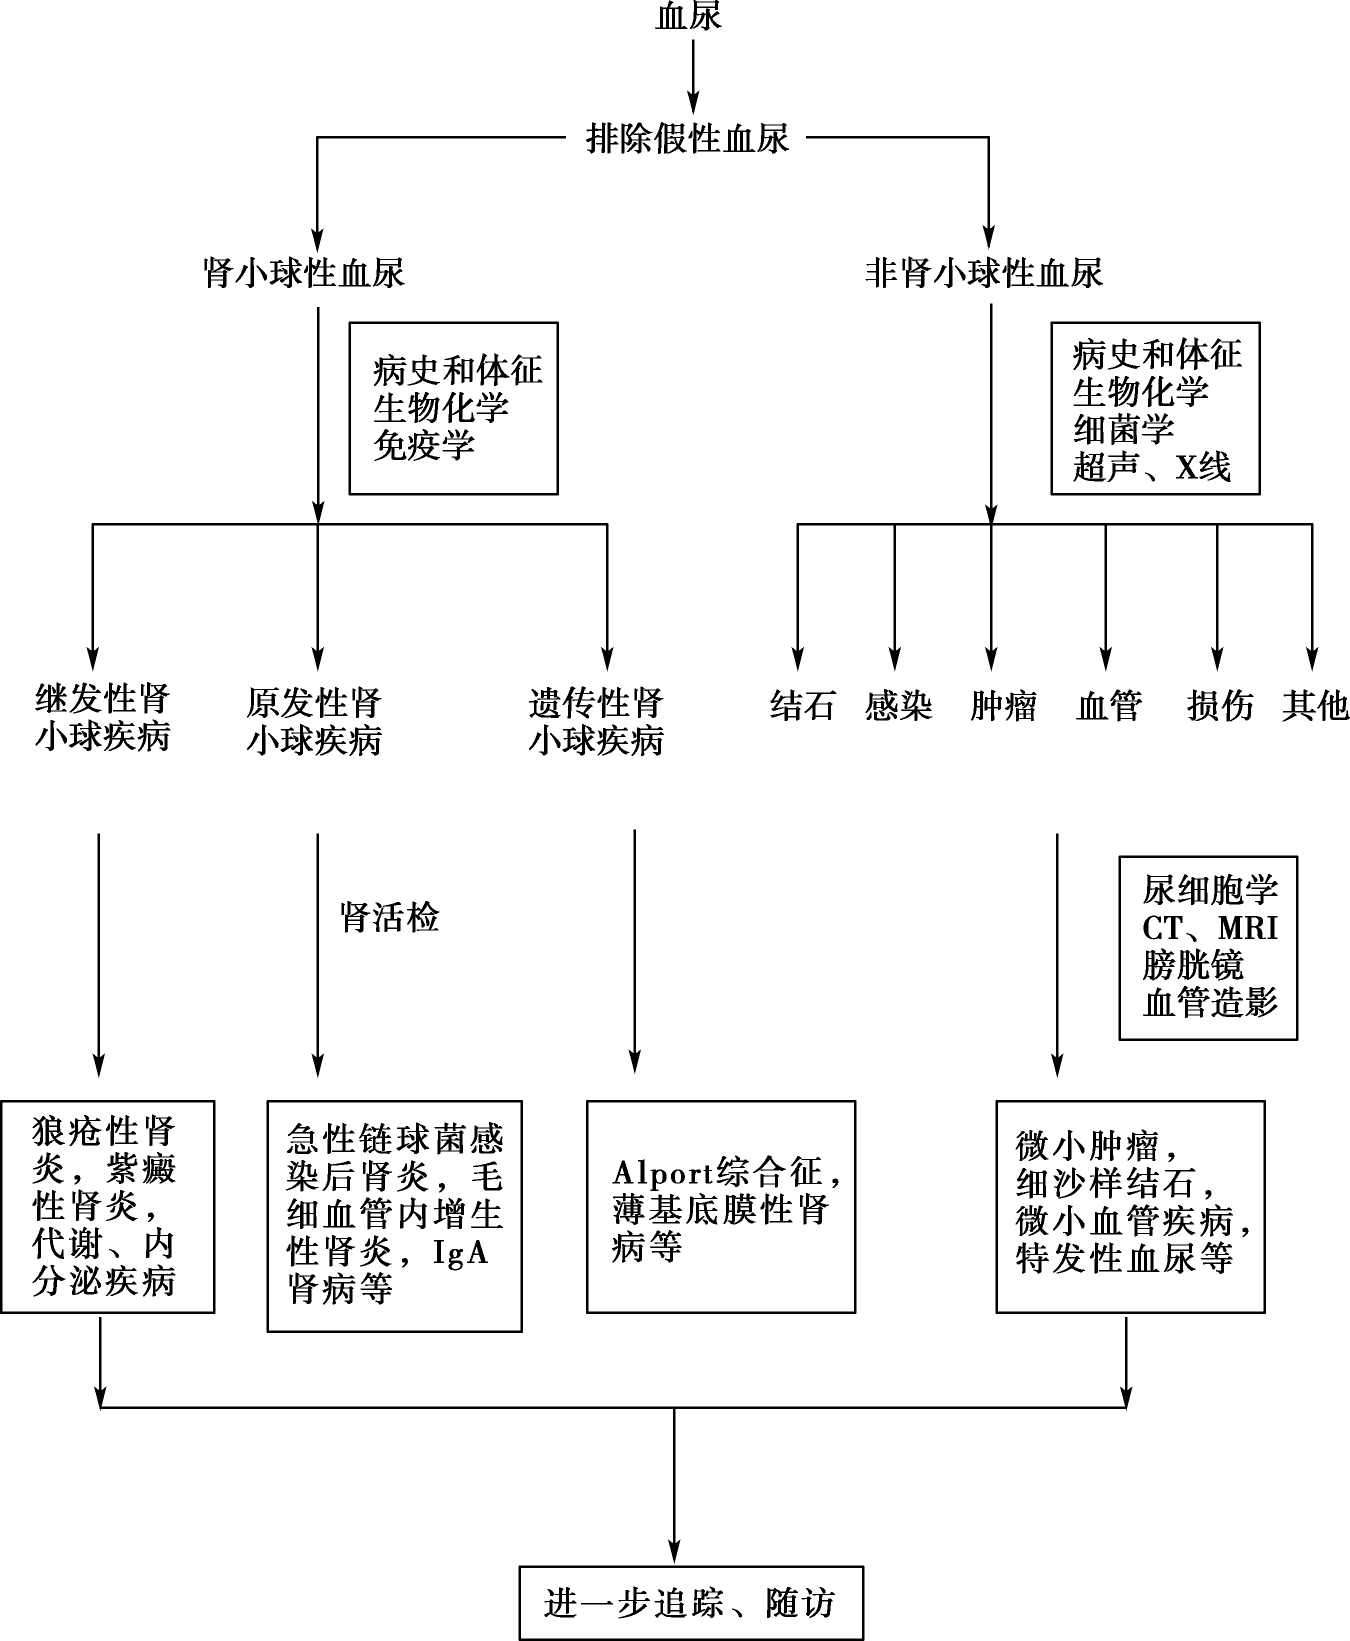
\includegraphics[width=4.6875in,height=5.58333in]{./images/Image00223.jpg}

血尿的诊断程序

\begin{table}[htbp]
\centering
\caption{血尿的原因及疾病}
\label{tab36-1}
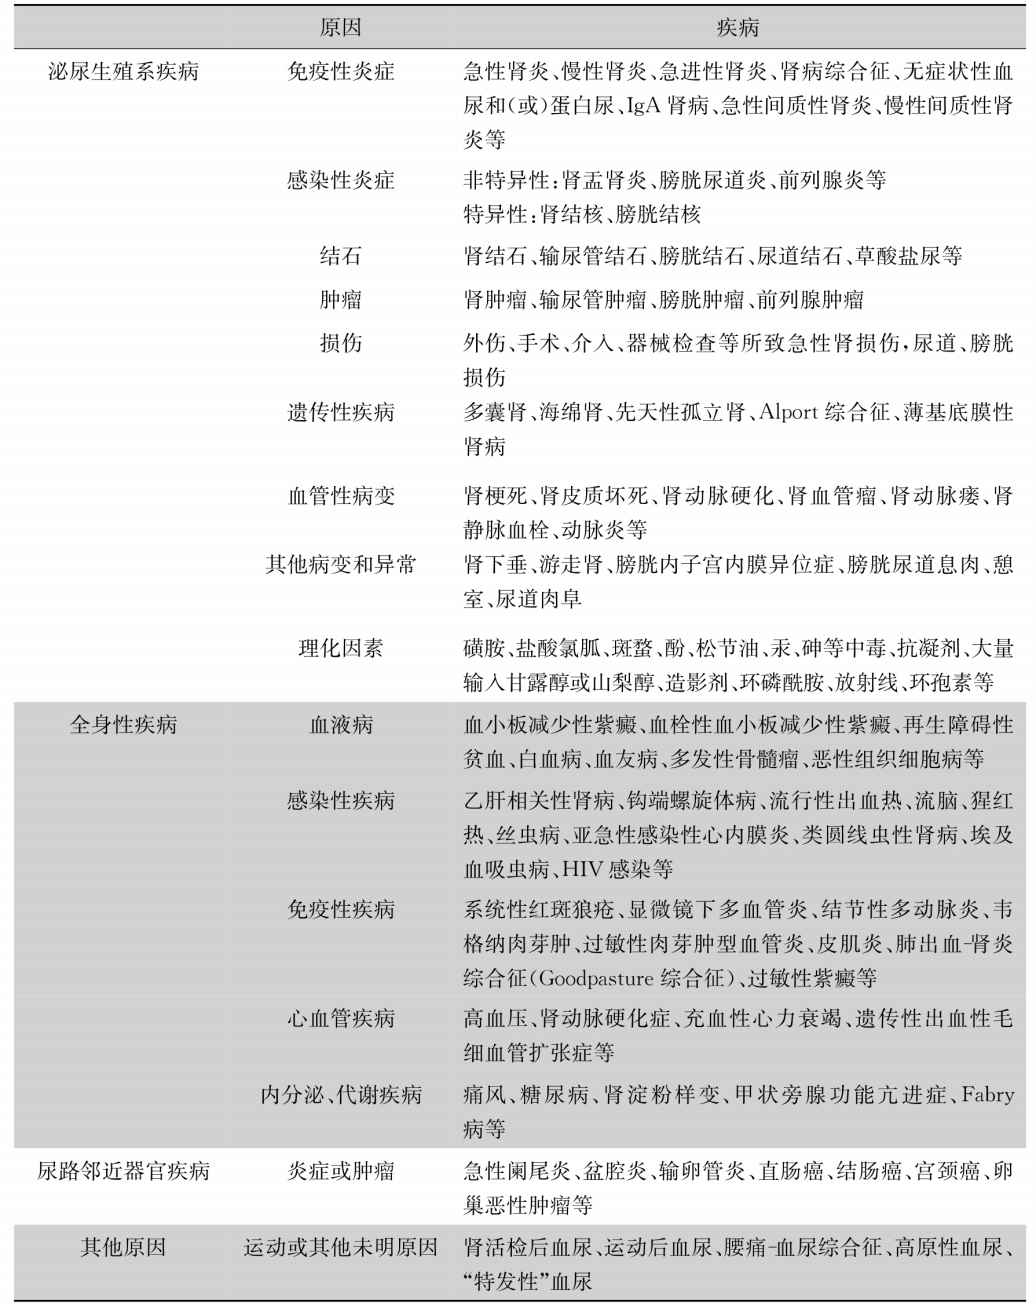
\includegraphics[width=5.95833in,height=7.52083in]{./images/Image00224.jpg}
\end{table}

\protect\hypertarget{text00277.html}{}{}

\subsection{119.1 泌尿生殖系疾病}

\subsubsection{一、免疫性炎症}

主要是原发性肾小球疾病和间质性肾炎。

原发性肾小球疾病(primary glomerular
diseases)是指不明原因导致的双侧肾脏弥漫性或局灶性肾小球病变。具有:①肾小球性蛋白尿(以白蛋白为主)伴管型尿和(或)肾小球性血尿;②肾外表现为高血压及水肿;③肾小球滤过功能损害先于并重于肾小管功能障碍的临床特点。原发性肾小球疾病常合并肾小管间质炎症性病变,是发展为肾衰竭的主要原因和影响因素。血尿可呈持续性镜下血尿和(或)反复发作性肉眼血尿,尿血细胞常以小细胞和畸形红细胞为主,可有红细胞管型。

原发性肾小球疾病的分类:通常有临床和病理分型:

\paragraph{(一)原发性肾小球疾病的临床分型}

根据症状、体征和生化检查分为

1.急性肾小球肾炎(acute glomerulonephritis)。

2.急进性肾小球肾炎(rapidly progressive glomerulonephritis)。

3.慢性肾小球肾炎(chronic glomerulonephritis)。

4.无症状性血尿或(和)蛋白尿(隐匿性肾小球肾炎)[asymptomatic hematuria
and(or)proteinuria]。

5.肾病综合征(nephrotic syndrome)。

\paragraph{(二)原发性肾小球疾病的病理分型(表\ref{tab36-2}):}

\begin{table}[htbp]
\centering
\caption{1995年世界卫生组织(WHO)关于原发性肾小球疾病的病理学分类}
\label{tab36-2}
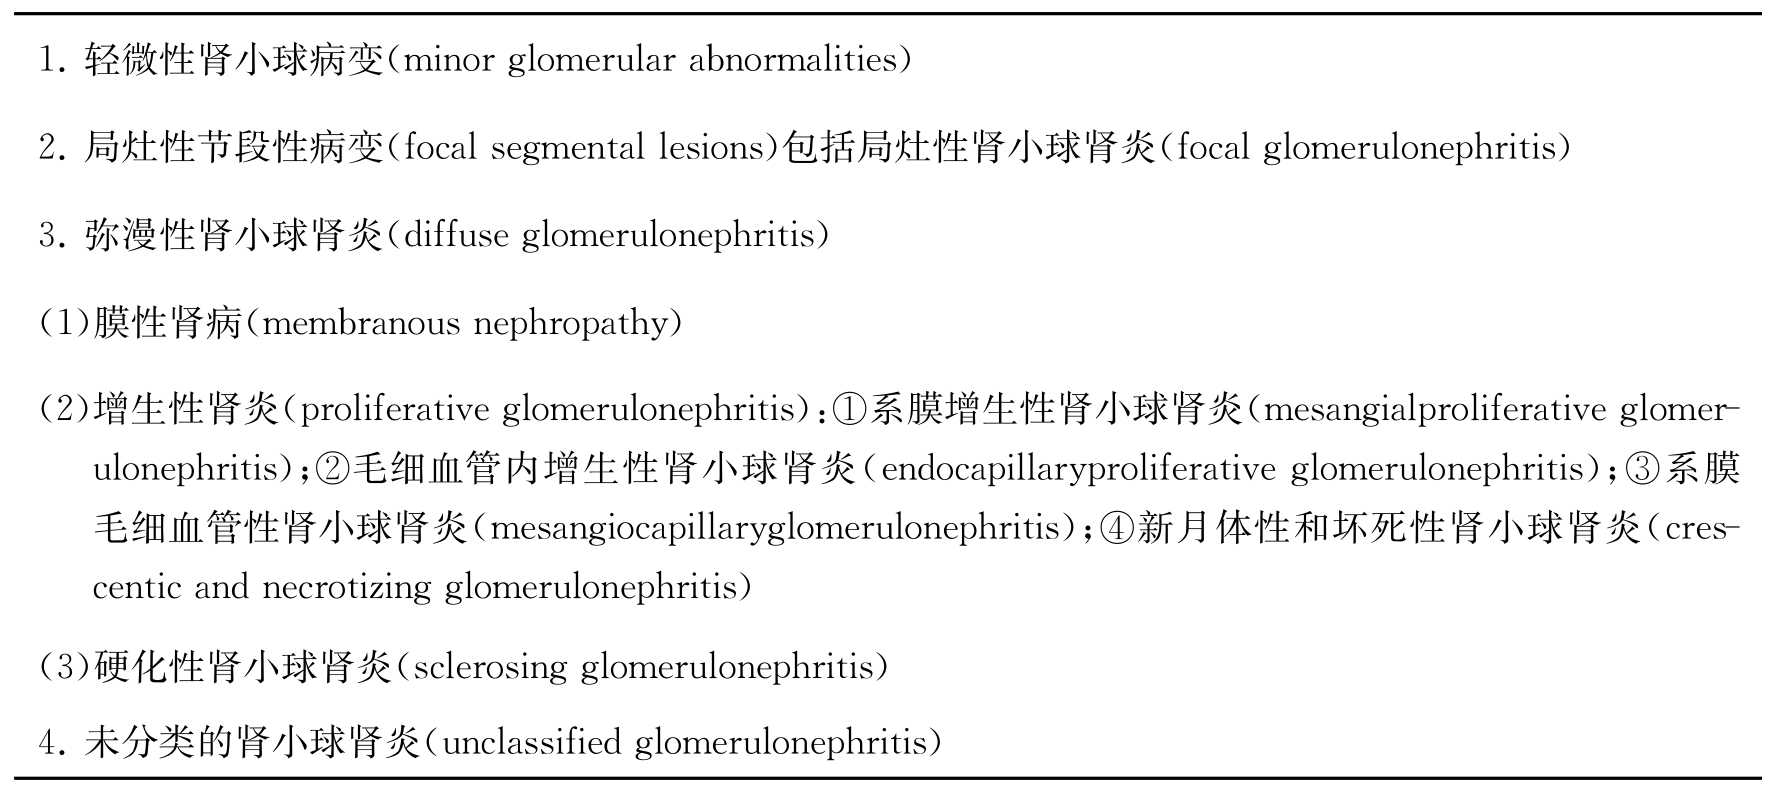
\includegraphics[width=5.91667in,height=2.61458in]{./images/Image00225.jpg}
\end{table}

继发性肾小球疾病是指全身或系统性疾病引起肾小球损害,如糖尿病或系统性红斑狼疮等。临床表现与特发性者相同,但有其原发疾病的各自特征。发作期均可出现血尿,重者呈肉眼血尿。但血尿不是这类肾炎的主要或唯一症状,常伴有蛋白尿、高血压、水肿及肾功能损害等。病因包括系统性疾病、血管性疾病、代谢性疾病、遗传性疾病等,根据临床、生化、免疫学和肾活检,多数能诊断(表\ref{tab36-3})。\footnote{这个分类将致密物沉积病从原发性肾小球疾病划为继发性肾小球疾病。但是,目前多数学者倾向于将IgA肾病归于原发性肾小球肾炎}

常见的以血尿为主要症状的原发性肾小球疾病:

(一)急性链球菌感染后肾小球肾炎
又称为毛细血管内增生性肾小球肾炎(简称急性肾炎),本病可见于各个年龄组,以儿童和青少年好发。大部分患者有前驱感染病史,咽部感染后的潜伏期为7~21天,平均为10天。皮肤感染后的潜伏期长一些,约为14~21天。临床多表现为急性肾炎综合征,也可表现为急进性肾炎和肾病综合征,病情严重程度波动很大。

\begin{table}[htbp]
\centering
\caption{1995年世界卫生组织(WHO)关于继发性肾小球疾病的分类}
\label{tab36-3}
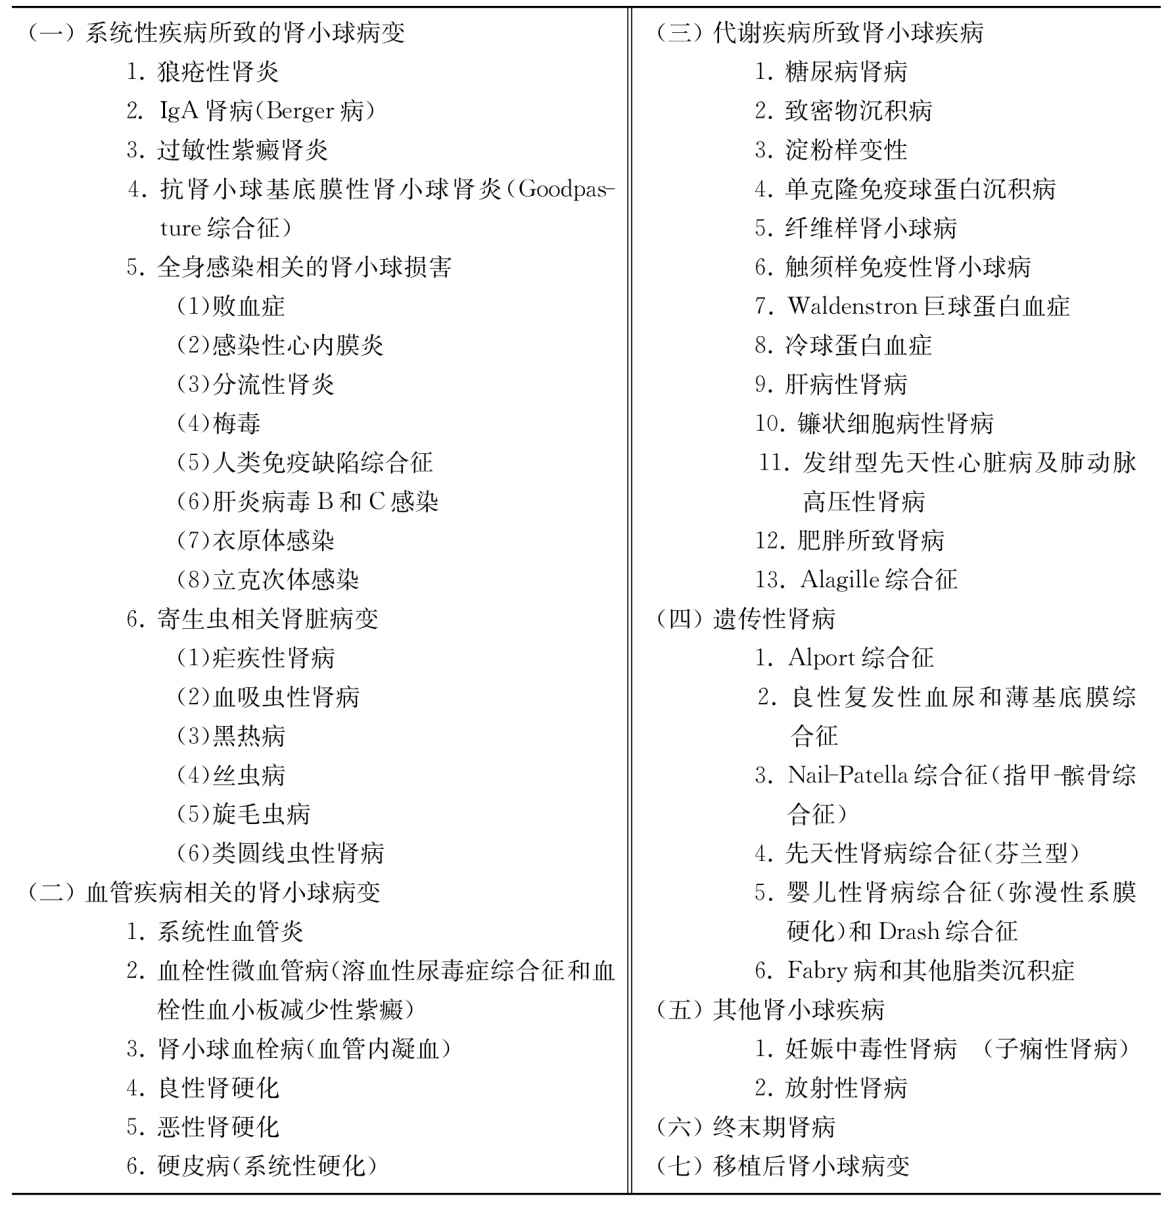
\includegraphics[width=5.91667in,height=6.10417in]{./images/Image00226.jpg}
\end{table}



血尿常为本病的首发症状,几乎所有患者都有血尿,约40\%患者有肉眼血尿。严重者可有尿频和尿道不适,数天至两周即消失,但无典型的尿路刺激症状。尿中无血凝块,镜下红细胞少数可迁延数月至1~2年。血尿通常伴有短暂的少尿或无尿,偶尔这种状况持续存在,则提示有新月体形成。较轻的亚临床病例,可全无水肿、高血压和肉眼血尿,仅仅尿常规发现镜下血尿,有时尿检也正常,仅血中C3呈典型的急性期明显降低,而6~8周恢复。此类患者行肾活检可见典型的毛细血管内增生及特征型的驼峰样改变。

(二)IgA肾病
IgA肾病是一种免疫复合物介导的肾小球肾炎,以肾小球IgA沉积为主要特征,可表现为不同类型的病理改变。IgA肾病约占所有原发性肾小球疾病的20\%~40\%。早期认为IgA肾病是一种比较良性的肾脏病,但现在发现高达20\%~40\%的患者最终可发展至肾衰竭。IgA肾病好发于青年男性,发病年龄多见于20~30岁之间,IgA肾病主要表现为血尿、蛋白尿、氮质血症和高血压等。约30\%~50\%IgA肾病可表现为发作性血尿或持续性镜下血尿。血尿常表现为两种类型:①发作性肉眼血尿:此型约占所有IgA肾病的40\%~50\%;常于上呼吸道感染后数小时或1~3天后发生肉眼血尿,偶有胃肠道感染后或运动后血尿发作,儿童患者80\%以上可有肉眼血尿,成人则只有40\%左右发作肉眼血尿。②持续性镜下血尿:本型约占所有IgA肾病的30\%~50\%,无明显肉眼血尿,镜下血尿持续存在,可伴有蛋白尿,可见于各种年龄段。

IgA肾病的病程个体差异较大,多数患者病情呈慢性进行发展,可多年表现为良性血尿和正常肾功能,部分表现为急进性肾小球肾炎,肾功能急剧恶化和终末期肾衰。个别IgA肾病可在病理改变较轻和临床表现呈良性过程的基础上,突然出现毛细血管袢坏死和新月体的形成,病理上表现为新月体肾炎,并伴有较严重的肾小管-间质病变。这些患者与上述病理改变较轻的急性肾功能不全临床上不容易鉴别。一般地,对于无症状血尿患者(不伴有血压升高及血肌酐升高者),不主张积极进行肾活检检查。中山医一院肾内科资料显示:表现为单纯性血尿的IgA肾病病理改变比较轻,78.6\%患者病理分级为Lee氏Ⅰ~Ⅲ级,但仍有20.4\%患者为Ⅳ~Ⅴ级,提示这些患者虽然临床表现轻,但病理分级可以相当严重,显示病理和临床可能存在不一致性。因此,单纯血尿伴在下列情况时:①24小时尿蛋白排泄量大于1.0g/d或表现为肾病综合征;②血肌酐升高;③血尿明显伴短时间内血肌酐升高;④伴有高血压;⑤怀疑继发于全身性疾病肾小球疾病,如糖尿病肾病、狼疮肾炎或肝炎相关性肾炎等;⑥怀疑合并其他肾小球疾病,应该进行肾活检:对于没有行肾活检者,临床上必须密切观察,出现上述指征时应及时肾活检,为临床上采取针对性措施提供依据。

(三)系膜毛细血管性肾小球肾炎(MCGN)又称膜增殖性肾小球肾炎(MPGN)
本病开始时,患者几乎总有血尿,包括镜下或者肉眼血尿。血尿常为镜下持续性血尿,约有10\%~20\%患者常于呼吸道感染后呈发作性肉眼血尿,为严重的、尿红细胞多样畸形的肾小球性血尿。本病25\%~30\%表现为急性肾炎综合征,30\%表现为无症状性蛋白尿,50\%的患者表现为肾病综合征,90\%以上患者蛋白尿选择性差。约30\%以上患者伴有高血压。患者常于起病后即有较严重的正细胞正色素性贫血,并且贫血的程度与肾功能减退程度不成比例。至少有半数的患者出现急性或慢性肾功能不全。

本病的一个特征性改变就是血补体的降低,约有75\%的本病患者C3持续性降低。尿FDP和C3可升高。原发性肾小球疾病,除链球菌感染后肾炎外,少见C3降低。由于该病常表现为急性肾炎综合征,常可有前驱呼吸道感染史,40\%在起病前有抗“O”滴度升高和链球菌感染的其他证据。故应与链球菌感染后肾小球肾炎相鉴别。毛细血管性肾小球肾炎补体持续降低,多大于2个月。与本病不同,链球菌感染后肾小球肾炎的C3水平常下降,但在6~8周多恢复到正常水平。而持续的低补体血症则应怀疑该病。并且链球菌感染后肾炎的病理常表现为毛细血管内增生性肾小球肾炎,结合肾活检的病理检查不难区分两者。因此,持续性的低补体血症,持续无选择性的蛋白尿(或肾病综合征)伴有严重的多样变形的红细胞尿,与肾功能下降不成比例的贫血,常提示该病发生。

继发于狼疮性肾炎、晚期肝病、单克隆球蛋白病、白血病和转移癌的肾病综合征可以出现C3下降,病理检查有时与本病有些混淆,但是注意结合临床其他表现和免疫荧光检查的C\textsubscript{1}
q的阳性程度以及血清免疫学等检查可加以鉴别。其他糖尿病肾小球硬化或者轻链沉积病有时光镜改变相似,但是免疫荧光和电镜的结果可以容易地将本病和其他疾病区分开,结合临床表现,血生化和血清免疫学检查就更容易鉴别。与其他的继发性系膜毛细血管性肾炎相鉴别。如乙肝相关性肾炎,根据病毒血清学及肾脏组织乙肝病毒抗原标志物可以鉴别。冷球蛋白血症临床与病理均与该病相似,但很少见,并且前者有相应的全身表现,病理有肾脏小血管炎和透明血栓形成提示为继发性的病变。

常见的几种感染后发作血尿的疾病的鉴别(参见表\ref{tab36-4})。

\begin{table}[htbp]
\centering
\caption{三种肾小球肾炎伴血尿的鉴别}
\label{tab36-4}
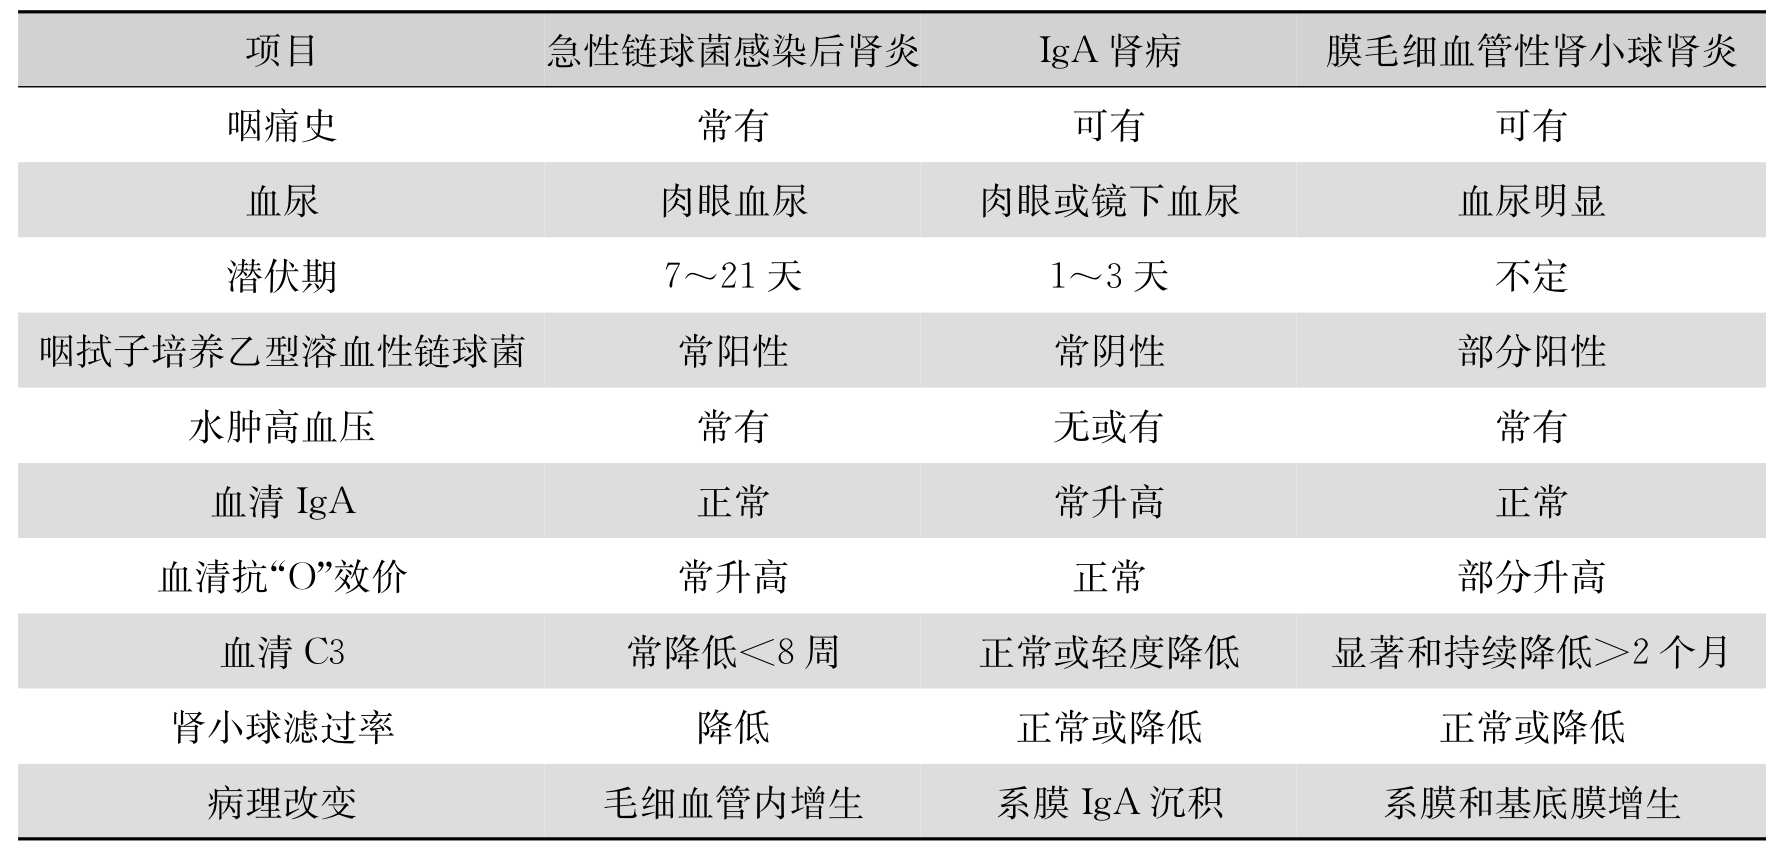
\includegraphics[width=5.95833in,height=2.84375in]{./images/Image00227.jpg}
\end{table}

(四)系膜增生性肾小球肾炎(MsPGN)
MsPGN是以病理形态特征为肾小球呈弥漫性系膜细胞增生和(或)不同程度的系膜基质增多,伴或不伴IgG,C3系膜沉积而毛细血管壁正常的一组肾小球疾病。MsPGN可见于任何年龄,以儿童和青少年多见,男性稍多于女性,男性与女性之比为1.5∶1至2.3∶1,国外本病在原发性肾综中,成人占10\%,儿童占15\%,在我国成人中约占30\%,40.3\%的患者病前有前驱上呼吸道感染症状。

MsPGN常隐匿发病,临床表现可为孤立性血尿、无症状性蛋白尿、蛋白尿合并血尿,60\%~70\%的患者可有镜下血尿,偶有肉眼血尿,肉眼血尿发生率为IgA肾病的1/3~1/2。59\%表现为肾病综合征,肾病综合征的发生率是IgA肾病1.5~3.0倍。本病国外报道事先常无激发或感染因素,但国内北京和上海有学者报道部分患者有前驱感染病史。约20\%~40\%患者有轻中度高血压,其与病变程度有关。肾功能一般正常,重度系膜增生可发展为慢性肾功能不全。部分肾病综合征患者血清IgG水平轻度减低,约30\%的患者血清IgM水平升高,补体水平正常,极少数患者有C4水平下降,有些患者可有含IgM或IgG的循环免疫复合物,ASO滴度正常。

(五)微小病变肾病
微小病变肾病好发于儿童,大部分患者起病隐匿,无明显诱因。少部分患者起病前有上呼吸道感染史(多为不典型病毒感染)或过敏之后,或有药物反应史,如非甾体消炎药、干扰素、青霉素及异胭肼等,血尿发生率约15\%~20\%,儿童血尿少见,成人较多血尿。水肿常为首发症状,多有大量蛋白尿和肾病综合征。病理检查肾小球基本正常,无免疫复合物沉积及电子致密物,电镜下肾小球上皮细胞足突弥漫性融合。临床上很难区分轻微系膜增生性肾小球肾炎与微小病变肾病。MsPGN好发于青少年,血尿发生率为60\%~70\%,病理检查肾小球具有轻度系膜细胞及基质增生,有免疫复合物沉积于系膜区,电镜检查部分病例见电子致密物。有学者认为,微小病变肾病可演变成MsPGN,此二种病理类型是同一疾病的不同阶段,两者均可并发局灶性节段性硬化。

(六)局灶性节段性肾小球硬化
局灶性节段性肾小球硬化(FSGS)临床上主要表现为肾病综合征或慢性肾炎综合征。血尿比微小病变常见,大约有一半患者有镜下血尿,但肉眼血尿则少见。局灶性节段性肾小球硬化大多数临床表现为肾病综合征,成人50\%以上呈肾病综合征的表现,常伴有肾功能的减退,约有1/3就诊时有肾功能不全。在诊断FSGS时,应注意各种可能的继发性因素,如HIV感染、吸毒、肥胖等。病理检查见局灶性节段性肾小球硬化及玻璃样变,IgM及C3呈团块状沉积于病变部位上,电镜发现弥漫性肾小球脏层上皮细胞足突融合。FSGS有时误诊为微小病变,主要是由于FSGS的病变呈局灶性分布,肾活检时可能没有取到有节段性硬化或玻璃样变的肾小球而漏诊。鉴别FSGS和微小病变具有重要意义,因为前者对糖皮质激素的敏感性不如后者,常需要较大剂量和较长疗程的糖皮质激素进行治疗。此外,需与MsPGN鉴别,MsPGN有约30\%的病例表现为肾病综合征,20\%~30\%的病例表现为肾炎综合征,肾功能的减退较少见。病理表现为肾小球弥漫性系膜细胞及基质增生,IgG/IgM及C3呈颗粒状弥漫沉积于系膜区,以肾综大量蛋白尿为表现的患者电镜检查见有足突融合。重度MsPGN病例,在肾小球的某些节段上系膜基质亦可呈高度结节状增多,周围毛细血管腔塌陷,出现局灶性节段性硬化。

(七)急进性肾炎
急进性肾炎可有前驱感染,起病急,主要表现为血尿、蛋白尿等肾炎综合征的表现,但突出的表现是肾功能急剧恶化和进行性少尿或无尿,并很快发展为尿毒症。肉眼血尿比较常见,但蛋白尿呈轻至中度,一般不表现为肾病综合征。本型是我国最常见的新月体肾炎,主要见于青少年,血中可检测到免疫复合物,血补体C3可降低。总体来说,可分为原发性急进性肾炎和继发性急进性肾炎,继发性急进性肾炎多继发于SLE、Goodpasture综合征、ANCA相关性血管炎和过敏性紫癜等。Goodpasture综合征、ANCA相关性血管炎的患者可有咯血、气促和肺出血等肾外表现,系统性红斑狼疮有其他全身性症状和原发病的表现。急进性肾炎的患者大多数为免疫复合物型急进性肾炎。10\%~20\%患者血中有抗GBM抗体。少数为寡免疫复合物型急进性肾炎,常常有ANCA阳性,该型的临床和病理改变比抗GBM型和非免疫复合物型要稍轻。

对于临床上呈急性肾炎综合征表现的患者,如果出现肉眼血尿,并有少尿或无尿、肾功能不全,应警惕急进性肾炎的可能。在排除了肾前性和肾后性梗阻等因素后,应及时行肾活检确诊。同时检查血抗GBM抗体、P-ANCA(MPO)或C-ANCA(PR3)。免疫荧光对进一步分型有重要作用,如果不能及时获得抗GBM抗体的检测结果,可根据免疫荧光IgG沿基底膜呈细线状沉积初步诊断为抗基底膜肾炎,及时给予血浆置换,以免延误治疗时机。肺出血死亡率高,应注意早期诊断,包括肺部X光片检查、痰吞噬含铁血黄素巨噬细胞的检查和血气分析等。对于突然发生的贫血应注意肺出血的可能。血补体C3降低提示继发于感染后肾小球肾炎、狼疮性肾炎、系膜毛细血管肾炎或冷球蛋白血症的肾损害。抗核抗体(ANA)和抗双链DNA(dsDNA)的检测有助于狼疮性肾炎的诊断。双肾B超检查有助于排除肾后性梗阻所致的急性肾衰竭和了解疾病的可逆性。本病还应注意与各种病因的急性肾衰竭及各种原发性肾小球疾病相鉴别。

\subsubsection{二、感染性炎症}

肾盂、输尿管、膀胱、尿道、前列腺、尿道旁腺的细菌或寄生虫感染,使尿路黏膜产生炎性病变,可引起镜下血尿,甚至肉眼血尿。下面重点叙述肾盂肾炎、肾结核、膀胱尿道炎及前列腺炎。

\paragraph{(一)肾盂肾炎}

一般情况下,肾盂肾炎引起血尿,以镜下血尿为常见。少数重症急性肾盂肾炎或慢性肾盂肾炎急性发作的患者,可产生肉眼血尿,称之为“出血性肾盂肾炎”。此外,患者常同时伴有畏寒、发热、明显腰痛和膀胱刺激症状,出现脓尿,尿培养细菌阳性等现象(参见第3节)。

\paragraph{(二)肾结核}

肾结核发病年龄最多在20~40岁之间,男性约为女性的二倍。早期病变约80\%以上侵犯双侧肾,以后绝大多数(约85\%以上)为单侧性;如为双侧性,则一侧往往较重。发病过程比较缓慢,早期常无特殊不适,只于尿常规检查时发现异常。据国内文献报道1011例肾结核临床分析,首发症状常为尿频(78.9\%)、血尿(77.6\%)和尿痛(46.3\%),而且进行性逐渐加重,这是由于脓液刺激或结核杆菌侵犯膀胱所致。血尿可来自肾脏或膀胱,但以后者为主,故临床上多呈“终末血尿”,少数可呈大量全程血尿;因此血尿和尿频对本病的诊断有相当重要性。此外,患者多伴有肺结核或其他肺外结核,约有50\%~80\%的肾结核的男性患者伴有男性生殖系统结核,因此附睾结核在肾结核患者中是常见的。附睾结核可发生于肾结核出现症状之前或同时,故可作为肾结核诊断的线索。同时所有患者几乎都有不同程度的全身性结核中毒症状,如微热、盗汗、衰弱、贫血等。在诊断上,典型病例一般不难。有下列情况者则提示肾结核的可能性。

(1)肺结核或肺外结核(尤其附睾结核)患者,如有血尿出现,则有肾结核存在的可能;如同时伴有膀胱刺激症状,则可能性很大。

(2)患者有慢性逐渐加重的膀胱刺激症状,出现脓血尿,尿呈强酸性反应,尿沉渣镜检所见以红细胞为主,而尿普通细菌培养反复多次为阴性(阳性也不能排除,因可合并感染),用普通抗菌药物治疗无效者,应考虑肾结核的可能;如为男性患者,则可能性更大。

(3)青、壮年人(40岁以下)出现无其他症状的严重血尿,应考虑肾结核的可能。

(4)单侧的慢性腰痛而伴有原因未明的间歇发热,如同时有尿改变者。应考虑肾结核的可能。

如有上述情况,应按常规步骤进行24小时尿沉渣直接涂片抗酸染色,找寻结核杆菌[注意与耻(包皮)垢杆菌区别],阳性率约70\%。必要时可作尿结核杆菌培养与豚鼠接种(阳性率达约90\%),这对肾结核的确诊有决定性意义。其他可有结核菌素(PPD)皮试、血PPD
IgG、PPD
IgM检查有助于诊断。在怀疑病例未能确诊时,可进行静脉肾盂造影检查;如仍未能确定,则进一步作膀胱镜检查,可见膀胱黏膜充血、水肿、结核结节或结核性溃疡等,同时可进行逆行肾盂造影术;据国内统计,91\%的病例逆行肾盂造影可发现典型的结核性破坏现象,但只有42.5\%的患者能作这种造影。X线照片上的典型改变为,肾盏阴影模糊、变形、边缘不整齐如虫蛀状或破坏缺损,严重者可见空洞形成、肾盂狭窄、变形;输尿管呈节段性狭窄、僵直、变形等。少数钙化型肾结核,在X线腹部平片上可见钙化阴影,但需注意与肾结石、肾肿瘤等所致的钙化影区别。肾结石阴影位于肾盂、肾盏内,密度均匀,呈完整结石状,而肾结核的钙化影在肾实质。密度不均匀,呈斑点状。

肾结核与慢性肾盂肾炎非常相似,均可出现血尿和膀胱刺激症状,但后者出现血尿时多数在急性发作阶段,伴有畏寒、发热,出现明显脓尿,膀胱刺激症状为间歇反复发作性,时轻时重。尿普通致病菌培养阳性,菌落计数10万个/毫升或更多,但找不到结核杆菌。亚硝酸盐还原试验,肾盂肾炎呈阳性反应(约80\%),而肾结核则阴性,但肾结核并发感染时也可呈阳性,故只对单纯肾结核才有一定的鉴别意义。此外,肾盂肾炎用一般抗菌药物治疗常奏效,而对肾结核无效。

肾结核也常与慢性非特异性膀胱炎(尤其是女性患者)相似。后者常以脓尿为主,膀胱刺激症状时轻时重,无全身中毒症状/普通尿培细菌阳性。尿中找不到结核杆菌。

有时肾结核又与膀胱结石或膀胱肿瘤相混淆;后者在膀胱刺激症状出现之前已先有原发病的表现,如大量血尿、排尿困难等。

肾结核引起的无痛性血尿须与肾肿瘤区别,但后者血尿多较严重且为全程血尿,有肾肿块,发病年龄多在40岁以上。

少数肾结核患者因血块或脓块通过输尿管时,引起单侧肾绞痛,与肾结石相似,但后者绞痛先于血尿,或与血尿同时出现。如输尿管完全梗死引起结核性肾积脓形成巨大肾肿块时,则须经超声波检查、细菌学检查、肾图、X线肾盂造影或CT、MRI检查;才能与肾肿瘤、肾积水、腹腔内或腹后壁肿瘤等相鉴别。

肾结核发病潜隐,经尸解证实的病例,仅20\%生前作出诊断。临床诊断病例多属晚期,早期诊断率仅6\%。早期患者可无症状,而尿中常有结核分枝杆菌排出。但由于排菌量少,常规方法不易检出。PCR技术检测尿标本中结核菌,敏感性为90\%,但特异性和稳定性不高,而PCR仍存在着假阳性与假阴性的问题,目前较少使用。用ELISE法检测者血清中结核抗体,敏感性为87\%,与PCR技术相似,但特异性比PCR更强,可作为一项有价值的辅助诊断方法。

\paragraph{(三)膀胱尿道炎}

本病是最常引起血尿的疾病。女性多见,尤以生育期妇女为多。血尿多为终末血尿,严重者可呈全程血尿,同时伴有明显膀胱刺激症状,如尿频、尿急及尿痛等。发病多为急性,也可呈慢性而反复急性发作。此病常易被误诊为肾结核、肾盂肾炎等。本病一般无发热,很少有腰痛,肾功能正常,尿改变有时无,阴道指检压尿道有脓液流出,脓液培养细菌阳性等可资鉴别。

骨髓移植后出血性膀胱炎:近年渐多报告。研究材料表示与骨髓移植类型、腺病毒感染的移植物抗宿主病等因素有明显的相关性。有报告一组发生率为23.3\%(14/60)。B超检查为无痛性、无创伤、简便、快速的方法,可作为出血性膀胱炎的常规检测手段。

\paragraph{(四)前列腺炎}

本病也是引起血尿的一种常见而易忽略的疾病。多为终末血尿。必须强调,原因未明的血尿患者,虽患有前列腺炎,而前列腺炎不一定是血尿的病因。

\subsubsection{三、泌尿系结石}

\paragraph{(一)肾、输尿管结石}

肾、输尿管结石是常见的疾病。任何年龄均可发生,但多在20~50岁之间。男性多于女性。典型的临床表现为突发性肾区绞痛,呈刀割样痛,且沿输尿管行径向下放射至同侧阴部,甚至同侧大腿内侧;也有呈间歇性或持续性肾区钝痛者。在疼痛发作期间或发作后出现不同程度的血尿,镜下血尿多于肉眼血尿。少数无尿路梗阻的肾、输尿管结石患者可呈无痛性血尿,故青壮年人运动后出现无痛性全程血尿,首先应除外肾结石。急腹症患者尿常规检查,如尿中有红细胞,也应考虑肾、输尿管结石的可能性。对怀疑为肾结石而尿常规检查阴性时,在患者病情许可的情况下,可嘱患者按耐受程度作适当的跳跃运动,然后再作尿常规检查,如发现尿液中有红细胞存在,则提示泌尿系结石的可能。过去有肾绞痛、血尿、排尿石史是重要的诊断根据。

B超和X线检查是诊断肾、输尿管结石的重要方法。绝大多数(约95\%)患者在腹部B超和平片上可显示结石的致密阴影,但少数(5\%)由于结石太小或为可透X线的结石(如尿酸石)而呈阴性。因此,B超和腹部平片无结石阴影发现也不能完全排除结石的存在,应进一步作静脉肾盂造影。腹部平片上的结石阴影,应注意与肾钙化灶、钙化淋巴结、静脉石、阑尾炎结石、肠结石、粪石或骨岛等相鉴别。必要时可作静脉肾盂造影(在肾功能尚好的情况下)或逆行肾盂造影。血和尿的钙和尿酸定量测定对诊断也可有所帮助。在诊断上要着重于全面的临床综合分析,不要单凭X线检查来决定,因为不恰当的选用X线检查或不正确的X线造影技术,常常造成诊断的错误。对X线检查阴性或在未做X线检查时,可嘱患者在肾绞痛发作后,每次排尿时注意有无砂石排出,如有砂石排出,则为泌尿系线结石的有力证据。

少数无痛性血尿的肾结石常需与肾结核、肾肿瘤相区别。后两者以无痛性肉眼血尿为主,血量较多,且常于自发性血尿之后发生肾绞痛,乃因血凝块或脓块排出堵塞输尿管所致;此外,尚有原发病的临床表现以供临床鉴别诊断。

有时不典型的右侧肾、输尿管结石的临床表现与胆石症和急性阑尾炎相似,甚至误诊而进行手术,应注意鉴别。胆石症不引起血尿;盲肠后位阑尾发炎时可波及右输尿管而引起轻微镜下血尿,直肠指检有助于鉴别。

偶尔肾结石患者表现腹部锐痛、呕吐、腹胀和排气停止等症状,与急性梗阻相似,须与各种原因所致的肠梗阻区别。肠梗阻一般无血尿,腹部平片及尿常规检查有助于鉴别。

肾、输尿管结石常伴有膀胱刺激症状,尤其输尿管下1/3段的结石更明显。如同时并发感染或继发膀胱结石,则膀胱刺激症状更严重,常误诊为急性或慢性肾盂肾炎、急性膀胱炎等。相反,对经久不愈的肾盂肾炎,尤其是有复杂细菌感染者应考虑肾结石共存的可能。此外,还需注意与膀胱肿瘤相鉴别。部分急性前列腺炎合并精囊炎患者,可引起类似肾石绞痛的临床表现,也需注意区别。

还有少数双侧输尿管结石患者,病程长,无绞痛,临床表现与慢性肾炎后期、尿毒症相似,故对于不典型的后期慢性肾炎患者,如无明显的肾炎病史,代谢性酸中毒和氮质血症严重,经常有血尿而无明显蛋白尿及管型尿的患者,应作X线腹部平片检查以排除双侧输尿管结石阻塞的可能。

\paragraph{(二)膀胱结石或尿道结石}

膀胱或尿道结石多由肾、输尿管结石下降而来,也可原发于膀胱或尿道。老年人和10岁以下的男童较为多见。由于肾结石对膀胱、尿道黏膜的刺激、损伤可引起出血,因此血尿是其主要症状。膀胱与后尿道结石多呈“终末血尿”,有时滴出数滴鲜血。此外,患者常有耻骨上或会阴部钝痛或剧痛,明显的尿频、尿急、尿痛;患者于排尿时常排出小石等。探子探查、肛门指检、X线照片检查有助于诊断;极少数为可透X线的结石,需作膀胱镜检查或膀胱造影才能确诊。

\paragraph{(三)草酸盐尿}

草酸盐尿阻塞及损伤肾小管引起血尿者文献有报告。国外文献报道有些患者的症状与尿路结石相似,尿沉淀有大量草酸钙结晶与红细胞,尤其进食大量西红柿、菠菜之后易于发生,但症状在运动后不加剧,X线检查也未能证明尿路结石的存在。其中以血尿为主。但也有无痛性者。好了部位为输尿管下段,常累及膀胱。膀胱镜检及X线尿路造影术对此病的诊断有重要帮助。如X线肾盂造影显示肾积水而原因未明时,应考虑此疾病的可能性。

\subsubsection{四、泌尿系肿瘤}

\paragraph{(一)输尿管息肉和膀胱肿瘤}

输尿管息肉也甚少见。主要症状为血尿,多为间歇性无痛性血尿。其次为肾区痛及腹部肿块,乃由于输尿管阻塞引起肾积水所致。因息肉不易产生完全阻塞,故腹部肿块多不明显。X线肾盂造影和膀胱镜检查对诊断有帮助。常与输尿管原发肿瘤难以鉴别,但后者常为恶性,而息肉为良性。

膀胱肿瘤在泌尿系统中很常见,可分为原发性和继发性。原发性可分为膀胱上皮细胞性与非上皮细胞性肿瘤两大类,绝大多数为上皮细胞性肿瘤(97.5\%)。膀胱上皮细胞性肿瘤男性多于女性,发病年龄绝大多数在40~60岁之间,多发生于膀胱三角区及两侧壁。血尿为最常见和首发的主要症状,呈肉眼血尿或镜下血尿,但以肉眼血尿多见;为持续性或间歇性,可为“初始血尿”,也可为“终末血尿”或全程血尿,有时排出血块;晚期由于肿瘤增大、坏死或继发感染,引起膀胱刺激症状;也可由于肿瘤或血块阻塞尿路而致排尿困难,产生急性尿潴留。在诊断上,有人报告40岁以上大量血尿患者,约有半数以上是由于膀胱肿瘤所致。对于中年以上血尿或伴有膀胱刺激症状的患者,如体格检查不能发现明显的上泌尿系的病变,应考虑膀胱肿瘤的可能性。需进一步作膀胱镜检查或膀胱造影术以明确诊断。尿的细胞学检查可能有助于膀胱上皮细胞性肿瘤的诊断。临床上常需与肾结核和泌尿系结石相区别。

\paragraph{(二)前列腺肿瘤}

前列腺肿瘤多见于老年人(50岁以上),可分为良性(即前列腺肥大)和恶性(即前列腺癌),均可发生血尿。血尿轻重不一,可为肉眼血尿,也可为镜下血尿,为间歇性,多数出现于排尿后,呈“终末血尿”。前列腺肥大早期可无特殊症状,但在血尿发作前多有较长时间的尿频、排尿困难病史,血尿多因感染所致。经常发作肉眼血尿者,常为并发膀胱结石所致。前列腺癌早期的临床特点与前列腺肥大相似,发生血尿者占10\%,后期常伴有背或腰部疼痛的恶病质现象。

直肠指检是重要的诊断方法。绝大多数前列腺肥大和前列腺癌患者均有前列腺增大,指检时可触及。前者质呈中等硬度,有弹性感;后者则质坚硬,结节状且固定,如硬结很大则诊断当无问题,如硬结较小则需与前列腺结核或结石相区别。血清酸性磷酸酶测定前列腺癌多增高,有转移者更明显(不增高不能除外),但非特异性。血清前列腺特异性抗原(PSA)测定,诊断意义较大。作肛门、直肠前列腺活检诊断明确。

\paragraph{(三)肾脏肿瘤}

肾错构瘤在不同年龄均可发生,可有腹痛,镜下血尿等,B超、CT可明确诊断。

\subsubsection{五、遗传性肾脏病}

\paragraph{(一)遗传性肾炎(Alport综合征)}

遗传性肾炎(也即Alport综合征)是一种遗传性疾病,在文献中它被称为遗传性肾炎、遗传性进行性肾炎、家族性出血性肾炎、遗传性慢性肾炎。血尿是本病常见而首发的症状,且从幼年即出现,其他临床主要表现为神经性耳聋、眼疾和慢性肾功能不全,同时存在三种损害的病例少于5\%,男性的病情比女性重,有家族病史。肾组织电镜病理检查见肾小球基底膜广泛变厚、劈裂,并与变薄的GBM并存,与薄基底膜性肾病明显不同。

\paragraph{(二)薄基底膜性肾病}

本病也称“良性”家族性血尿,多数有家族史,但也见于非家族性血尿患者。任何年龄均可发病,以中青年多见。上呼吸道感染剧烈运动后可呈现肉眼血尿,无链球菌感染的证据,这与链球菌感染后急性肾炎不同。临床上以反复发作性血尿为特征,儿童可仅为无症状单纯性血尿,成人可有少量蛋白尿,不伴有水肿与高血压,也无肾功能损害,患者镜下血尿可持续很长时间,预后良好。

肾活组织检查光镜下常无明显病理改变,偶也可见轻度局灶性肾炎的表现。电镜下基底膜弥漫性变薄(成人基底膜<265nm,儿童基底膜<250nm)而无电子致密物可确诊。

\subsubsection{六、其他泌尿系疾病}

\paragraph{(一)肾下垂或游走肾}

肾下垂是指患者在吸气时检查者用双手可触到半个以上肾脏者;游走肾则指患者的肾脏能在腹部各方向自由活动者。本病多见于瘦长体型的女性,多数发生于右侧肾。有时可由于肾静脉暂时性弯曲以致肾淤血或继发肾盂感染而引起血尿。患者主要症状为腹部包块,肾区于劳动或站立后疼痛(卧床休息后好转),需与腹部其他肿块,肾肿瘤,肾结石、肾结核等所致的肾积水,先天性多囊肾等相区别。X线肾盂造影(平卧与站立位比较)可明确诊断。

\paragraph{(二)先天性肾异常}

\subparagraph{1.先天性多囊肾}

此病是由于先天性肾发育异常所致的疾病。部分患者以血尿为主征,血尿轻重不一,常为间歇性。此病多在35岁以后发现。多囊肾绝大多数为双侧性,可较正常肾增大2~6倍,故可触及两侧增大的肾脏,表面不平滑,稍有囊样感。肾区常感钝痛,偶可引起绞痛,大部分患者伴有高血压。晚期有包块进行性增大的同时,出现进行性肾功能不全。临床上如遇有原因未明的血尿、肾区痛、高血压、触及肿大的肾脏(双侧)、有肾衰竭的表现者,则先天性多囊肾的可能性很大,早期常常误诊为肾肿瘤、肾结核、肾结石、游走肾、单囊肾、肾包虫囊肿及腹部其他肿瘤等,需注意鉴别。B超肾区检查,提示肾区多个囊性包块;肾盂造影见肾盂变长、变窄,肾盏呈新月形压迹;CT等检查对本病诊断有重要意义。

\subparagraph{2.海绵肾}

海绵肾为先天性疾病。乃由于肾集合管呈囊状或梭形扩张,肾锥体内出现很多囊腔而呈海绵状所致。本病多发现于40岁以上的男性。病变多为双侧性(约占80\%),少数为单侧或局灶性。本症的临床特征:早期可无任何症状,但由于本病容易并发结石或感染,故可有血尿、尿路阻塞、肾绞痛及泌尿系感染症状等,病程中可出现高血压。本病多为泌尿系X线检查所发现。静脉肾盂造影可见到类似海绵状、葡萄状、花朵状及分枝状影。如囊腔内合并结石时,在X线平片中可见到相当于肾髓质部位有多数小钙化影,并于多次检查可发现钙化影的排列发生改变。

\subparagraph{3.先天性孤立肾}

此病是由于胚胎时期一侧生肾组织或输尿管芽发育障碍所致的一侧肾缺如。占肾畸形的15\%。患者常以血尿为主诉,但一般无症状。如发现一侧代偿性肿大的肾脏,即应考虑先天性孤立肾的可能,但须与肾肿瘤或其他腹部包块相区别。B超、X线肾盂造影、CT有助于诊断。

\paragraph{(三)膀胱内子宫内膜异位症}

此病是由于子宫内膜异位于膀胱内黏膜所致。以周期性血尿为主诉。血尿与月经来潮有明显关系,经期过后血尿即停止。此外还有膀胱刺激症状。

\subsubsection{七、理化物质或药物对泌尿系统的损伤}

肾、输尿管、膀胱、尿道等受外伤、器械检查或手术等,均可引起创伤出血而出现血尿。可根据病史、体征以及其他有关检查以确定损伤部位。

磺胺类药物引起的血尿临床上有报告,尤其大量静脉注射更常见。主要由于其晶体沉积于肾小管内,阻塞及损伤肾小管所引起。其特点为尿沉淀中有大量磺胺晶体。棉酚、斑蝥、酚、鱼胆汁、松节油、汞、砷、抗凝剂、环磷酰胺、放射线、异物等可损害肾脏或膀胱而致血尿。大量甘露醇或山梨醇静脉注入,也有引起血尿的报告。之外,近年来报道的中药马兜铃酸相关的肾损害也可有血尿。此类血尿的特点是:有应用化学药品或药物史,血尿为短暂性,停药则可自愈。

\protect\hypertarget{text00278.html}{}{}

\subsection{119.2 全身性疾病}

\subsubsection{一、血液病}

如血小板减少性紫癜、再生障碍性贫血、白血病、血友病、恶性组织细胞病等可因血小板减少、毛细血管通透性增加和凝血机制障碍等因素而引起血尿。多发性骨髓瘤也可伴蛋白尿、血尿。此外,患者全身各处均可出血。诊断时可根据各原发病特征进行鉴别。此外,近年来也注意到血浆性病因引起血尿。这是由于尿液中的尿激酶促使前纤维蛋白溶酶形成纤维蛋白溶酶,再作用于纤维蛋白,使其溶解而引起凝血机制障碍所致。对原因未明的血尿应考虑血液病的可能。应用6-氨基己酸等止血药治疗可奏效。

\subsubsection{二、感染性疾病}

如钩端螺旋体病、流脑、流行性出血热、猩红热、亚急性细菌性心内膜炎、天花等均可引起血尿,但多见于严重感染患者,诊断时可根据各原发病特征进行鉴别,原发病治愈后血尿消失。

丝虫病所致的乳糜血尿在丝虫病区常见。此类患者如尿中含乳糜不多,以血尿为主时,常被误诊为膀胱肿瘤或其他泌尿系疾病。因此,在诊断时应予以注意。详细询问病史可获得过去有过乳糜尿或丝虫病感染史。人类感染是由于进食含该虫幼虫的生鱼肉或半生鱼肉引起。乙肝相关性肾炎,HIV感染也可发生血尿,蛋白尿。HIV感染要了解有吸食毒品史。

\subsubsection{三、风湿免疫性疾病}

\paragraph{(一)系统性红斑狼疮(SLE)}

SLE是一种自身免疫性疾病,可累及全身多个系统,血清中出现多种自身抗体和循环免疫复合物(CIC),并有明显的免疫紊乱。SLE出现肾损害者,则为狼疮性肾炎(lupus
nephritis,LN)。

SLE女性多见,男女之比为1∶13,但男女患者有同样高的肾脏受累率,平均发病年龄约为27~29岁,85\%的患者年龄在55岁以下。SLE是一种全身性疾病,可累及多个系统和脏器,约70\%的患者有肾脏损害的临床表现,结合肾活检组织免疫荧光和电子显微镜检查,则SLE100\%有肾脏累及。狼疮性肾炎的临床表现多样,起病可隐袭也可急骤,症状可轻可重。可仅为单纯性血尿和(或)蛋白尿,也可出现明显的肾病综合征或肾功能损害。常因感染、受凉、日光照射、酗酒、应激、过度劳累或精神紧张等到因素导致疾病发作或加重,也可因激素应用不当,减量过快或骤然停药而引起复发。每一次复发,都会使受累的脏器损害更为加重,甚至出现功能衰竭。狼疮性肾炎累及的症状几乎包括肾小球,肾小管间质和肾血管损害的一系列症状,水肿很常见,1/6的患者在确诊时有肾功能不同程度的下降。

SLE多见于青、中年女性,大多数患者可出现全身乏力,体重下降、消瘦的表现,90\%的患者有发热,其中65\%作为首发症状。热型不定,可为间歇热、弛张热、稽留热或慢性低热。40\%可超过39℃,应注意是否因感染所致,特别是应用大剂量激素治疗的患者。SLE常有多系统、多器官受累。SLE的皮肤黏膜损害多种多样,发生率在80\%以上。50\%的患者可出现蝶形红斑,为鼻梁和双颧颊部呈蝶形分布的水肿性红斑(鼻唇沟处无皮损),可有毛细血管扩张和鳞屑,渗出严重时可有水泡和痂皮。红斑消退后一般不留瘢痕。20~30\%的患者可出现盘状红斑,多位于暴露部位的皮肤,为环形、圆形或椭圆形的红色隆起斑片,表面可覆有鳞屑及角质栓,皮损消退后常留有瘢痕。蝶形红斑和盘状红斑均为SLE的特征性皮损,日光或紫外线照射会加重。

35\%~58\%的SLE患者可有光过敏。50\%~71\%的患者可出现脱发,是SLE活动的敏感指标之一。约50\%的患者可出现血管性皮肤病变,为小血管及毛细血管炎症或痉挛所致。包括网状青斑、血管炎性皮肤损害、雷诺现象、甲周红斑、荨麻疹样皮损、冻疮样狼疮样皮损及毛细血管扩张等。7\%~14\%的患者可出现黏膜糜烂或无痛性溃疡。约95\%的患者可出现关节疼痛和关节炎,常见于四肢小关节。5\%~10\%的患者有无菌性股骨头坏死,多因长期、大量、不规则使用激素所致。SLE患者血沉快,γ球蛋白高,血中可出现多种自身免疫抗体,对诊断有重要意义。抗核抗体(ANA)阳性率高,达95\%,特异性约70\%,可作为良好的筛选试验;抗ds-DNA抗体阳性率约为72\%,特异性较高,可达96\%;抗Sm抗体:阳性率低,仅见于25\%的SLE患者,但特异性极高,可达99\%。肾活检结合免疫荧光和电镜检查,对SLE的确诊率几乎达100\%,并可确定狼疮性肾炎的病理类型及疾病的活动性和慢性变程度。

SLE的肾脏病变多种多样。其病理改变的特征为:①“铁线圈”样病损:由于内皮沉积物而使基膜增厚,电镜和免疫荧光检查有大量的内皮下沉积物,是SLE肾损害的重要特征;②苏木素小体:一般认为是抗核抗体在原位造成细胞损害所致,由高度凝固的细胞核染色而成;③坏死性血管炎:微动脉和毛细血管呈纤维素样坏死;④免疫荧光检查可见肾小球所有区域IgG、IgM、IgA、C\textsubscript{1}
q、C3、C4等呈颗粒状沉积,呈“满堂亮”现象;⑤电镜下可见电子致密物沉积、核碎裂、病毒样颗粒和包涵体。

典型的SLE诊断并不困难,但不典型或早期的SLE,须进一步与其他的风湿免疫性疾病鉴别、追踪随访,以明确诊断。

\paragraph{(二)过敏性紫癜(HSP)}

是一种伴IgA免疫球蛋白/复合物沉积于受累血管壁的血管炎临床综合征,主要表现为皮肤紫癜、黏膜出血、关节炎、腹痛及肾小球肾炎。本病肾脏受累的表现,称为过敏性紫癜肾炎,本病十分常见,国内报告在30\%~50\%。

HSP好发于2~10岁儿童,3~7岁为发病高峰,据统计,HSP肾炎在所有小儿肾小球疾病中约占15\%。成年人(>20岁)中少见,儿童患者中,男性好发,男女比例2∶1,成人患者无性别差异。本病好发生于寒冷季节,夏季发病率下降。大多数患者呈良性、自限性过程,多于数周内痊愈。但也有反复发作或迁延数月、数年者。约50\%患者病程反复发作。

发病有遗传易感性,与细菌与病毒感染,食物与药物过敏有关。约1/3患者有细菌、病毒等先驱感染史。细菌以β溶血性链球菌多见,但未能证明与链球菌感染的肯定关系。病毒感染常见的有风疹、水痘、流行性腮腺炎、麻疹、流感等。寄生虫感染是本病的常见诱因,有约1/4过敏性紫癜患者可找到相关诱因,可能与机体对寄生虫幼虫成长过程中的分解产物过敏所致变态反应有关。以蛔虫感染多见,约占3/4,其他有钩虫、鞭虫、丝虫、血吸虫、阴道滴虫、疟原虫等。

易过敏食物主要有鱼、虾、蟹、牛奶、鸡、鸡蛋等,可能由异体蛋白引起机体过敏所致。易过敏药物主要有常用抗生素(青霉素、链霉素、氯霉素、红霉素、磺胺类)、解热镇痛药(水杨酸类、氨基比林、保泰松、安乃近)、镇静药(苯巴比妥、水合氯醛、三氟拉嗪)、激素类(胰岛素、丙酸睾酮、人工合成雌激素)、抗结核药(对氨基水杨酸钠、异烟肼)、疫苗注射(结核菌素试验、乙肝疫苗),其他有洋地黄、奎尼丁、阿托品、麻黄碱、氯噻嗪、甲苯磺丁脲、丙硫氧嘧啶、奎宁、碘化物以及金、砷、铋、汞等。

其他诱发因素如寒冷、外伤、昆虫叮咬、花粉、内分泌紊乱、甚至精神因素等可诱发本病。起病可急可缓,50\%~90\%的儿童及30\%的成人于发病前1到3周内有上呼吸道感染、全身疲乏无力、纳差、低热等前驱症状。

所有患者均有紫癜性皮疹。特征性皮疹表现为大小不等、对称分布的出血性皮疹,多发生在四肢远端、臀部及下腹部,加压后不褪色,有痒感,1~2周后逐渐消退。常可分批出现,反复发作。约82\%患者出现多发性关节肿痛。多发生在踝、膝、肘等大关节。约25\%~63\%患者有腹部绞痛,常餐后加剧,伴有呕吐,可以并发呕血、黑便、稀便。孤立性镜下血尿是紫癜性肾炎最常见的临床表现,儿童患者出现肉眼血尿的较成人为多,这一症状通常是暂时的。当血尿持续存在,蛋白尿会逐渐增加,表现为慢性肾炎综合征,可伴有肾功能损害。成年人中10\%~25\%患者呈以急进性肾炎为表现的新月体肾炎,16\%~50\%呈肾病综合征表现。儿童患者表现为肾病综合征者稍微低于成人,约为8\%~32\%。

30\%~50\%患者束臂试验可阳性,3P试验可阳性,出、凝血时间及骨髓检查正常。约2/3患者血沉轻度增快,抗“O”一般不增高、血清总补体及补体C3一般正常。50\%~70\%患者血清IgA水平增高,可检出IgA型类风湿因子。抗中性粒细胞胞浆抗体(ANCA)一般阴性,但有时可发现IgG-ANCA阳性。紫癜性肾炎的特征性肾脏病理病变是系膜区广泛IgA颗粒状沉积并伴有巨灶和节段性增生性病变。

本病依靠临床典型的皮肤、关节、胃肠道及肾脏受累表现及IgA沉着为主的系膜增殖性病理改变,确诊并不难。因约25\%患者肾脏受累表现很轻,反复细致尿常规检查是检出肾受累的主要依据。本病需与小血管炎、IgA肾病等其他疾病进行鉴别诊断。

不同的小血管炎可出现相同的临床症状。例如,冷球蛋白血症性血管炎、显微镜下多血管炎、韦格纳肉芽肿、过敏性肉芽肿、狼疮性血管炎、类风湿血管炎和血清病性血管炎均可出现皮肤紫癜、腹痛、关节痛和肾炎,单靠临床表现难以进行细致区分。确诊需要免疫病理的进一步支持。临床具备上述小血管炎的症状和体征,如果血管壁或肾小球系膜区存在以IgA为主的免疫复合物沉积,可诊断为本病。如果存在相同临床表现,但存在循环冷球蛋白和血管壁存在冷球蛋白IgM、IgG颗粒沉积,可诊断为冷球蛋白血症性血管炎。如果具有相似临床表现,血管壁无免疫复合物沉积,但存在循环ANCA,则应考虑是否为寡免疫复合物性血管炎,这类小血管炎血管壁无或甚少免疫复合物沉积,包括显微镜下多血管炎、韦格纳肉芽肿、过敏性肉芽肿等疾病。

本病单根据肾脏病理与免疫病理的改变难以与IgA肾病相区别,但本病的肾小球毛细血管袢坏死及纤维素沉着的程度较重。IgA肾病不存在本病的肾外表现。且本病较多发生于儿童,呈急性疾病过程、病理改变大部分是非进行性的,其预后与起病时肾病理新月体的多少有关;而IgA肾病多见于成人,是一缓慢进展的慢性疾病,新月体形成并不明显,而节段性肾小球硬化较为突出。

在皮疹等肾外表现不明显时,应注意与急性链球菌感染后肾炎相鉴别,本病血清C3及抗链“O”滴度一般正常,而IgA及含IgA成分的循环免疫复合物等常可升高,注意检查肾外表现及必要时行肾活检均有助于鉴别诊断。

\paragraph{(三)原发性系统性血管炎}

血管炎是以血管壁发生炎症[包括炎性细胞浸润和(或)血管壁坏死]为特征的一组疾病综合征。血管炎分为继发性和原发性,继发性是指血管炎继发于另一种系统性疾病,如系统性红斑狼疮、感染、肿瘤等弥漫性结缔组织病,原发性是指无其他原因的系统性血管炎,又称为ANCA相关性血管炎,常见有显微镜下多血管炎(MPA)、韦格纳肉芽肿(WG)和过敏性肉芽肿型血管炎。目前,随着抗中性粒细胞胞浆抗体(ANCA)检查的开展,原发性血管炎的诊断率明显提高。

原发性血管炎临床上多见于中老年人,往往以原因不明的不规则发热、乏力、消瘦、皮疹、关节肌肉疼痛、腹痛、神经炎等非特异性症状出现。本病可累及几乎所有器官,最常见的是肾脏、皮肤、关节和肺等。肾累及者几乎均有血尿、肉眼血尿占1/3,蛋白尿较常见,部分患者可出现肾病综合征样病变。50\%患者出现急进性肾炎的临床表现,部分肾功能缓慢减退,部分患者有消化道症状或肺出血。

在鉴别诊断时要首先排除SLE、感染、恶性肿瘤和药物(肼屈嗪、丙硫氧嘧啶)等继发性因素引起的继发性血管炎。结缔组织病如系统性红斑狼疮、类风湿关节炎、干燥综合征等均可发生继发性血管炎,根据各自特有的临床表现和免疫学特征不难区别。其次,要注意与心黏液瘤、多发性胆固醇栓塞综合征等假性血管炎综合征以及细菌性心内膜炎、高血压性动脉炎、抗磷脂抗体综合征等鉴别。

某些临床症状往往能提示某一血管炎病,如鼻咽部血性及脓性分泌物常提示要注意韦格纳肉芽肿等。对于根据病史、体征及相关实验室检查不能确诊的病例,要考虑做血管活检或血管造影。皮肤活检对诊断一般不能提供很大帮助,肾活检对鉴别显微镜下多动脉炎和结节性多动脉炎有重要帮助。血管活检病理及血管造影结果要结合临床综合考虑。

显微镜下多血管炎主要累及小血管,肾脏受累常表现为急进性肾小球肾炎,部分患者出现肾功能不全,高血压不多见,肺受累主要表现为咯血、胸膜炎和哮喘,周围神经病变较为少见,ANCA阳性率较高,血管造影未见异常。出现下列情况时应考虑到显微镜下多血管炎的可能:①中年男性,存在系统性炎症性疾病的症状;②亚急性进行性肾功能不全;③肺出血,胸片示小泡状浸润影,需排除肺水肿或感染;④肾活检示系膜增殖和新月体形成的局灶节段性肾小球肾炎;⑤皮肤或其他内脏活检示白细胞碎裂性血管炎;⑥p-ANCA阳性。

原发性血管炎出现肺肾综合征时应与肺出血-肾炎综合征(Goodpasture综合征)相鉴别。后者多发于15~30岁,男性发病多见。发热、咯血及肾炎为其突出的临床特点,一般无系统性血管炎表现,抗肾小球基底膜抗体(GBM)阳性,而ANCA多阴性,肾脏病理原发性血管炎以血管的病变为主伴炎性细胞浸润,而肺出血-肾炎综合征可见IgG沿肾小球基底膜呈线状沉积。

结核性肉芽肿在临床和组织病理上与韦格纳肉芽肿(WG)有类似表现,但两者治疗截然不同,需注意鉴别,一般结核性肉芽肿常有结核菌素试验阳性,抗结核治疗有效。而典型的韦格纳肉芽肿可有上呼吸道炎症、肺部病变和肾小球肾炎三联症,血清C-ANCA是目前所发现的WG中最为特异的一个指标。

过敏性肉芽肿型血管炎患者过去常有支气管哮喘和(或)慢性呼吸道疾病病史,主要累及小血管及小静脉,常有肺血管损害,肾受累以坏死性肾小球肾炎为特点,嗜酸性粒细胞组织浸润,外周血象嗜酸性粒细胞增多,ANCA阳性率较高,可以鉴别。

如系统性红斑狼疮性、皮肌炎等,常常损害肾脏而产生血尿。此外,患者全身性多系统受累是此类疾病的特征。诊断时可根据全身多系统和各原发病特点进行鉴别。

肺出血-肾炎综合征(Goodpasture综合征)属于免疫性疾病,可能是由于肺及肾小球的毛细血管基底膜同时受免疫反应损害所致,但病因未明了。本病在临床上罕见。其临床特征是:反复咯血是首发症状,咯血常很严重,而导致呼吸困难及急性失血等表现,X线胸部检查见双侧点状或絮状阴影;于数天或数周后出现肾炎症状,血尿最常见,多为镜下血尿,也可有蛋白及管型尿,早期功能可正常,但病势发展迅速,一般于短期内产生尿毒症。抗肾小球基底膜抗体阳性,皮质激素冲击治疗,血浆置换治疗可有暂时缓解效果,但预后不良,常死于大量肺出血。

\subsubsection{四、心血管疾病}

高血压性肾损害、高血压动脉硬化并有高血压性肾病时,可引起镜下血尿;肾内小动脉破裂或肾小球出血时,可导致大量血尿。充血性心力衰竭也可因肾淤血而引起镜下血尿。遗传性出血性毛细血管扩张症也可引起血尿。近年心肾综合征的概念也明确心脏疾病和肾脏损害的相互关系。

\subsubsection{五、内分泌-代谢障碍性疾病}

痛风肾可引起血尿,血尿的轻重不一,主要是由于尿酸损害肾脏,或尿酸结晶通过尿路损害尿路黏膜所致。多见于晚期的老年痛风患者。在血尿出现之前多有反复发作的关节痛或皮下痛风结节等表现,血尿酸增高。

肾淀粉样变、糖尿病肾病也可引起轻度血尿,但较少见。根据原发病征不难鉴别。

甲状旁腺功能亢进症合并肾结石时可引起血尿。

\protect\hypertarget{text00279.html}{}{}

\subsection{119.3 尿路邻近器官疾病}

急性阑尾炎如炎症波及泌尿系统时可引起血尿,一般为短暂的镜下血尿。

女性盆腔器官发炎也可引起血尿。

直肠癌、结肠癌、宫颈癌、卵巢恶性肿瘤等均可侵犯泌尿系统而引起血尿。

可根据各原发病的特征进行鉴别诊断。

\protect\hypertarget{text00280.html}{}{}

\subsection{119.4 其他原因}

\subsubsection{一、肾活检后血尿}

经皮肾穿刺活检对肾脏病的病理诊断,指导治疗并提示预后均非常重要,目前,B超定位取材成功率很高,通常比较安全。但术后多有镜下血尿,少数有肉眼血尿,偶尔血尿相当严重提示可能穿到较大的血管。国内报道一组经皮肾穿刺并发症1000例中,重度血尿发生率0.4\%,严重时发生休克。文献报道出血发生率3\%~16\%,肾周围血肿发生率为5.2\%~7.8\%,有时血肿较大,个别需做肾切除。故术前需掌握适应证,禁忌证,术前检查出、凝血功能,控制血压,严格按B超定位方法及正规穿刺技术操作。

\subsubsection{二、运动性血尿}

有时健康人在剧烈运动后可出现血尿。其原因乃由于剧烈运动时肾脏血管床收缩,致肾脏血流量减少,氧供应暂时不足,致肾小球毛细血管壁的通透性增加,从而引起轻度的血尿。肾脏淤血、轻微外伤或膀胱也可能为引起血尿的原因;运动后血尿的特点为经休息后肉眼血尿很快转为镜下血尿和恢复正常,通常约需3~7天,除血尿外自觉良好,无其他系统性疾病,也无肾脏疾病的表现。

\subsubsection{三、腰痛-血尿综合征}

本病是一组以腰痛及血尿为表现的临床综合征。多见于应用口服避孕药物的青年妇女。病理检查:肾小球正常病变发生于叶间小动脉,荧光检查可见动脉壁C3沉着,但无免疫球蛋白沉积。临床特征为发作性肉眼血尿及一例或双侧腰部钝痛。可有少量蛋白尿,血压可升高,肾功能正常。肾动脉造影可见终末分枝动脉狭窄。停用口服避孕药可改善症状,预后未定。

\subsubsection{四、高原性血尿}

高原性血尿见于从平原进驻高原地区的人。此症诊断可根据:①患者有从平原进入高原史,或由低海拔进入更高海拔者;②有不同程度的高原适应不全症;③进入高原前或进入更高海拔前无血尿病史和泌尿系病史;④血尿发生于进入高原后,返回平原后血尿自行消失,而再次进入高原又复现血尿;⑤除外心、肾或其他系统性病变。

高原性血尿和高原性蛋白尿一般不单独存在,在急、慢性高原反应,高原红细胞增多症,高原肺水肿、高原昏迷,高原心脏病及高原高血压等高原病,均可造成肾小球滤膜受损,通透性增加,引起血尿或蛋白尿。高原性血尿的发生率与海拔高度无一定规律性,但随着移居时间的延长和活动量的增加而有所增加。高原地区出现血尿者,除了泌尿系统疾病及一些全身性疾病所引起外,尚有近1/2的血尿系高原性血尿,是高原病的并发症之一。在西藏的一项68例血尿患者的分析中,高原性血尿为23例。X线肾盂造影检查等影像学检查可作为一种辅助诊断的手段。

\subsubsection{五、“特发性”血尿}

临床上有少数以血尿为主诉的病例,患者全身状况良好,无泌尿生殖系统病变和全身或尿道邻近器官的病变,各项检查均未发现血尿的原因,可称为“特发性”血尿。约占血尿的6\%~8\%。

由于肾活检病理诊断的开展,许多以前临床诊断为“特发性”血尿已被发现是肾小球的轻微病变。如肾活检正常者,而出现较重的“特发性”血尿,可归纳为下列几种原因:①肾的小血管瘤或血管扩张;②肾盏-静脉通路;③微结石;④肾血管通透性增加性出血。大多数特发性血尿可能因肾淤血、血管神经功能紊乱、轻微的慢性炎症或过敏反应引起的肾血管通透性增加所致。在诊断时应注意体内有无感染病灶,病史中有无过敏性疾病,血尿与运动的关系,以及有无自主神经系统功能紊乱的临床表现。立位时作放射性核素肾图检查,注意肾脏血流量有无降低。详细观察泌尿系造影像,注意肾的位置、旋转度,以及肾盏、乳头、回流及钙化等微细的改变。上述资料对诊断“特发性”血尿有一定帮助,必要时还可作CT、MRI、血管造影并定期随诊。

\protect\hypertarget{text00281.html}{}{}

\section{120 血红蛋白尿}

尿内含有游离的血红蛋白称为血红蛋白尿,这是血管内溶血的证据之一。急性溶血时,血浆内的游离血红蛋白含量超过15~25mg/dl,则游离血红蛋白从肾脏排出,而发生血红蛋白尿。新鲜血红蛋白尿颜色粉红色,久置后在酸性环境呈酱油色,而在碱性环境下呈鲜红色。取新鲜尿标本离心、沉淀,镜检不见有红细胞或仅有少许红细胞,而联苯胺试验强阳性时,即可诊断为血红蛋白尿。

\subsection{【血红蛋白尿需与以下情况相区别】}

\subsubsection{一、卟啉尿(紫质尿)}

此尿也可呈暗红色或葡萄酒色,但联苯胺试验阴性,而尿卟胆原试验阳性。

产生卟啉尿主要是血卟啉病,但需与症状性卟啉尿相鉴别。引起症状性卟啉尿的疾病很多,如肝脏疾病(如肝硬化、肝癌、活动性肝炎等),血液病(如溶血性贫血、恶性贫血、再生障碍性贫血、白血病、红细胞增多症、血色病、淋巴网状细胞肉瘤等),糙皮病、高热和化学药物中毒(如铅、砷、硒、磷、双苯并蒽、磺胺、甲磺丁脉、巴比妥类、甲丙氨酯、利眠灵、鲁米特、苯妥英钠、麦角衍生物、氯霉素等)等。

\subsubsection{二、肌红蛋白尿}

肌红蛋白尿可发生在某些病理过程中所引起的肌肉组织变性、炎症与广泛损伤及代谢紊乱,致肌红蛋白自受损肌肉组织中渗出;肌红蛋白分子量小(17
500Da),易从肾脏排出而发生肌红蛋白尿,并可导致肾损害。

临床出现肌肉疼痛、无力,暗红色尿或棕黑色,伴严重肌肉损伤,严重时可有急性肾衰竭。确诊有赖于实验室检查。如尿液呈暗红色及联苯胺试验阳性而镜检无红细胞,血清肌酶(谷草转氨酶、乳酸脱氢酶、肌酸磷酸激酶)升高,而糖水试验阳性,Coombs试验阴性,则可能为肌红蛋白。肌红蛋白尿常需与血红蛋白尿相鉴别。血红蛋白不溶于硫酸铵,而肌红蛋白溶于硫酸铵;两者的分子量和等电点不同,在尿液蛋白电泳时,两者显示不同的电泳带可区别;肌红蛋白有肌肉症状,而血红蛋白有血管内溶血表现。

临床上肌红蛋白尿主要见于下列疾病:

(一)阵发性肌红蛋白尿 本病极罕见,国内尚无报道。患者可在运动后排出棕黑色尿,易与阵发性行军性血红蛋白尿混淆。本病患者表现特有的肌肉软弱无力乃至完全瘫痪,以及被动伸展时引起疼痛等症状,可作为两者的鉴别要点之一。

(二)挤压综合征 患者受挤压伤后有急性肾衰竭的临床表现,尿中测出肌红蛋白,可确立本病的诊断。

挤压综合征多由于意外事故,一肢体或多肢体经历数小时的严重挤压而致病。从损伤的肌肉渗出氧合肌红蛋白与变性肌红蛋白,并自肾脏排出。血液中肌红蛋白含量增高及休克,常导致急性肾衰竭。受伤严重的患者往往死于第六、七天间。尸检发现肾小管坏死,许多肾小管腔有肌红蛋白管型,肾小球似乎无改变。

(三)重度烧伤、电烧伤、大动脉血栓形成等 所致大块肌肉受损,也可引起肌红蛋白尿。

(四)“运动性”肌红蛋白尿。

(五)结缔组织病或感染 如皮肌炎、肌萎缩或急性多发性肌炎等。

(六)中毒 如海蛇咬伤,蜂毒,酒精中毒,纤维素厂所产生的化学毒物污染的鱼中毒(Haff病),海洛因中毒,两性霉素、甘草中毒等。

(七)MacArdle病 本病主要表现以运动后肌肉痉挛与乏力、间断性肌红蛋白尿、肌肉组织缺乏磷酸化酶活性为特征。

(八)其他
各种原因引起的动脉闭塞、剧烈痉挛或抽搐后、尿毒症酸中毒、低钾血症、急性全身性感染、恶性高热等。

\subsubsection{三、黑酸尿(alkaptonuria)}

黑酸尿罕见,国内仅有少数病例报告。此病可与血红蛋白尿相混淆。尿液长期暴露于空气中颜色变黑,提示本病,其原因是尿中有尿黑酸存在。患者有先天缺陷,根据“一基因一酶”假说,由于患者缺乏K基因,因而缺乏尿黑酸氧化酶,体内尿黑酸就不能转化为乙酰乙酸而从尿中排出。尿黑酸的存在可加碱以证明之:取患者新鲜尿液20ml,加10\%氢氧化钠溶液10滴,如有尿黑酸存在,尿液于30秒内逐渐由黄色→深黄色→红色,最后变为黑色。

尿黑酸长期积聚于身体各器官中,可引起褐黄病。黑色尿、皮肤棕黄色色素沉着与关节炎,是褐黄病独特的三联症。

\subsubsection{四、黑色素尿}

尿中含有大量黑色素可呈黑色,有时误为血红蛋白尿,需加区别。可见于广泛恶性黑色素瘤、慢性肾上腺皮质功能减退症、慢性肠梗阻伴有明显色素沉着等情况。有时服用左旋多巴、焦没食子酸也因药物色素而使尿呈黑棕色。

\subsection{【血红蛋白尿产生原因】}

主要有下列三项:

\subsubsection{一、在尿路中发生溶血}

血尿时如尿比重低于1.006,则红细胞在尿液中溶解,致形成血红蛋白尿(所谓假性血红蛋白尿)。

\subsubsection{二、肾梗死所致的血红蛋白尿}

肾梗死时可发生血红蛋白尿。溶血发生于梗死形成的肾实质区域内,血红蛋白从此处排入尿中。在单侧肾梗死时,膀胱镜检查可见棕色至深棕色尿从一侧输尿管排出,也有助于诊断。

上述两种情况极为罕见,其与血管内溶血的主要区别点为血浆游离血红蛋白与亲血色蛋白(haptoglobin)的含量均为正常。

\subsubsection{三、血管内溶血导致的血红蛋白尿}

此型血红蛋白尿最常见,其发病原因很多,是鉴别诊断的主要内容。分别讨论如下:

\paragraph{(一)先天性(遗传性)溶血所致血红蛋白尿}

如蚕豆病。

\paragraph{(二)后天获得性溶血性贫血所致血红蛋白尿}

\subparagraph{1.免疫性溶血性贫血所致血红蛋白尿}

(1)特发性慢性冷凝集素病:特发性慢性冷凝集素病常伴有手足发绀和肢端疼痛的雷诺现象,但国内报告引起血红蛋白尿者仅有一例。此病与阵发性寒冷性血红蛋白尿的溶血均由寒冷引起,两者的罗逊巴赫试验也可为阳性,临床上易混淆。其鉴别见表\ref{tab36-5}。

罗逊巴赫试验是将患者双手浸于冰水中10分钟,观察有无溶血现象发生。但此试验可能有危险性,一般不采用。

\begin{table}[htbp]
\centering
\caption{有血红蛋白尿出现的慢性溶血性贫血的鉴别诊断}
\label{tab36-5}
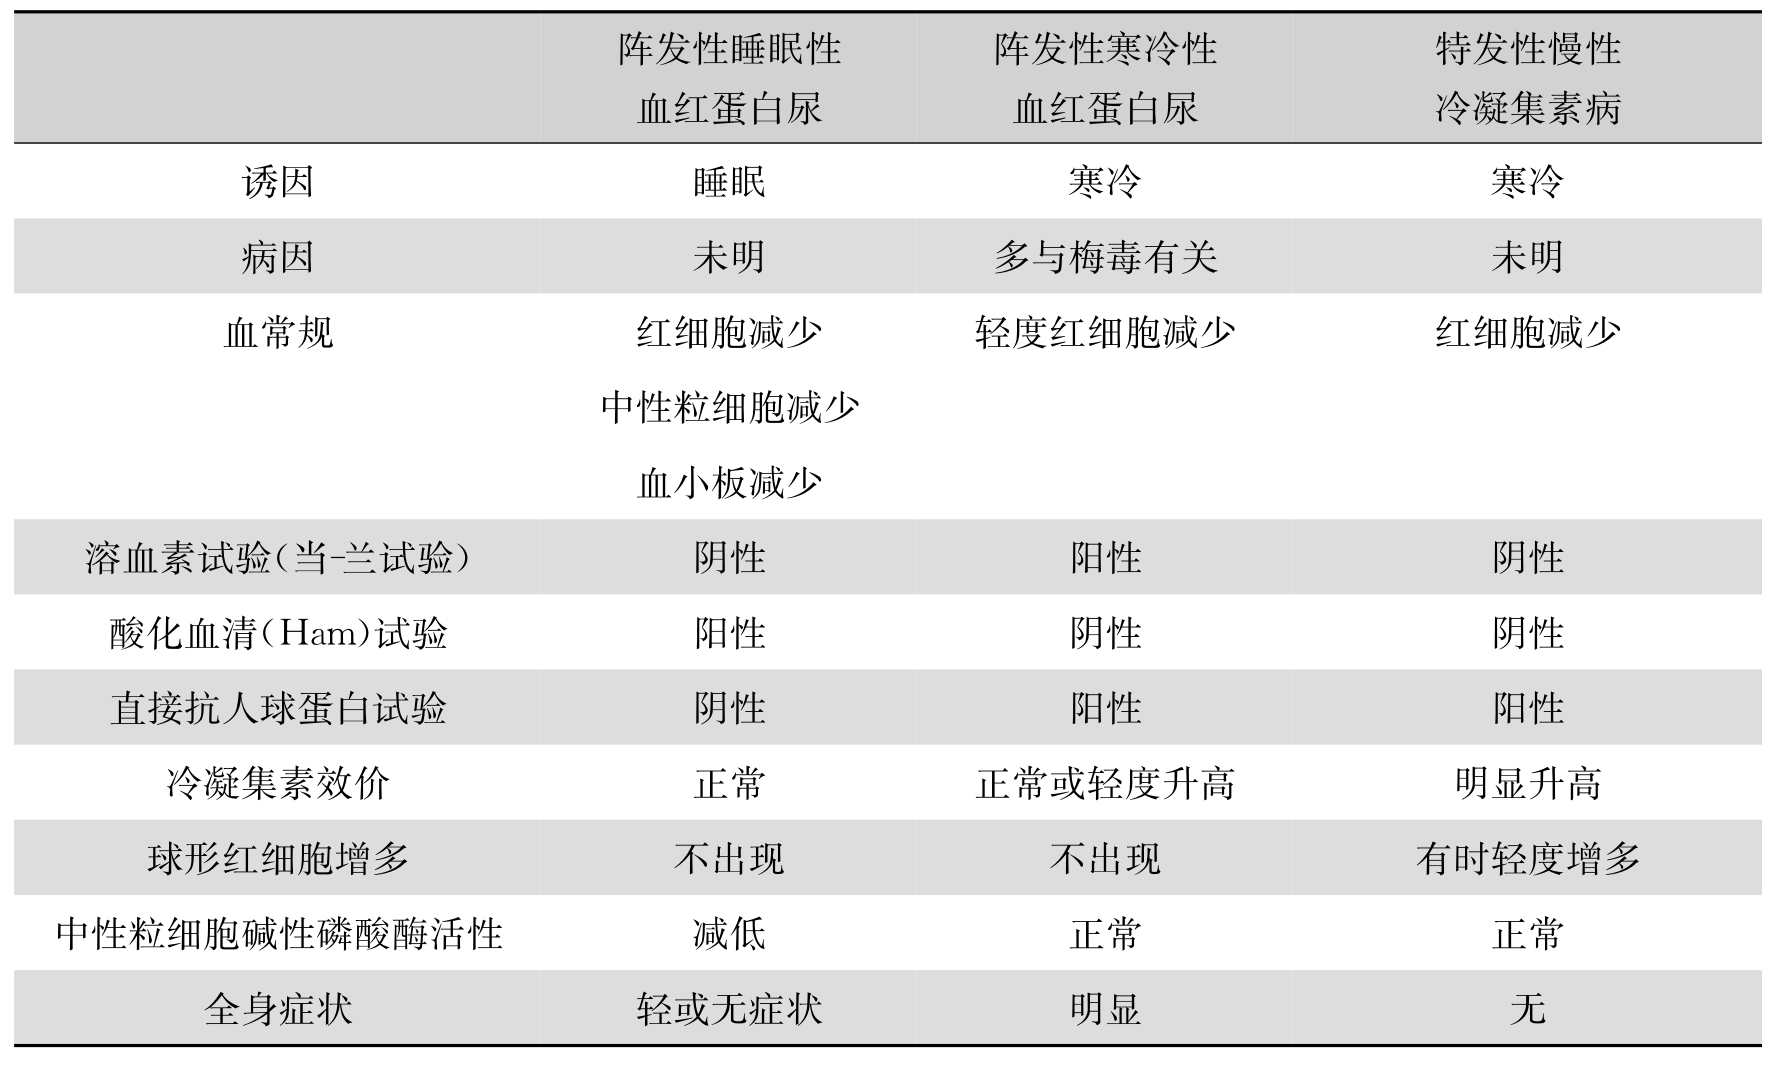
\includegraphics[width=5.9375in,height=3.54167in]{./images/Image00228.jpg}
\end{table}

(2)阵发性寒冷性血红蛋白尿较为少见,症状每因长时间暴露于寒冷环境中而诱发。

(3)血型不合溶血性输血反应所致血红蛋白尿。

\subparagraph{2.非免疫性溶血性贫血所致血红蛋白尿}

(1)药物或化学物品所致的血红蛋白尿:含砷的金属与稀硫酸成稀盐酸接触时,可产生砷化氢。砷化氢有高度毒性,吸入3~6小时后,可发生畏寒、头痛、腹痛、恶心、呕吐、软弱等症状,应考虑中毒的可能。如出现血红蛋白尿,则诊断可以肯定。

(2)感染所致的血红蛋白尿

1)黑尿热:黑尿热是一种急性血管内溶血现象。此病最多见于恶性疟疾区。患者以青壮年男性为多。发病最多由恶性疟引起,由间日疟及三日疟引起者甚少。如有疟疾发作,而后寒战发热与胆汁性呕吐及血红蛋白尿,提示本病的诊断。

2)伤寒并发血红蛋白尿:我院曾报道1208例伤寒患者中,有三例并发血红蛋白尿,均属男性患者,出现血红蛋白尿时间分别是病程的第3、11、13天。

(3)阵发性睡眠性血红蛋白尿:PNH主要典型表现为慢性血管内溶血。可有血红蛋白尿发作及贫血、黄疸等。但因本病临床的多样化表现极易误诊、漏诊。PNH的溶血机制,一般认为是由于睡眠时呼吸变浅,血中二氧化碳浓度增加,血pH值降低,在补体的作用下促使有缺陷的红细胞溶血。轻型病例可无血红蛋白尿发作,只有慢性溶血性贫血的表现。本病与阵发性寒冷性血红蛋白尿和特发性慢性冷凝集素病的鉴别诊断(参见表\ref{tab37-3})。

再生障碍性贫血-阵发性睡眠性血红蛋白尿症(AA-PNH)综合征:再生障碍性贫血和阵发性睡眠性血红蛋白尿症这两种疾病关系密切并可以互相转化,或同时存在。近年有报道在AA外周血及骨髓或单独从骨髓中检测出CD59\textsuperscript{-}
。细胞增多,虽然有关溶血试验阴性且无相关临床症状,但根据CD59\textsuperscript{-}
细胞增多可诊断为早期AA-PNH综合征。最新研究表明流式细胞术检测外周血粒细胞CD55、CD59和CD87有助于PNH、再障和骨髓异常增生综合征的诊断与鉴别诊断。

(4)阵发性行军性血红蛋白尿:患者有多次长跑后排出深棕色尿液的病史,提示本病的可能性。本病与阵发性肌红蛋白尿的主要区别点为:①后者有严重肌肉疼痛,而前者则不明显;②前者经长途步行或长跑后血浆游离血红蛋白明显上升而无肌红蛋白尿排出。

此病罕见,国内仅有少数病例报告。患者大都为青壮年男性战士或运动员,在长途行军或剧烈运动后两小时左右发生血红蛋白尿。发作血红蛋白尿之前常有全身不适与疲劳感,发作后腰部与下肢疼痛感、乏力等。个别病例可出现黄疸、肝脾大与贫血,或发生急性肾衰竭。根据血红蛋白尿仅发作于运动之后和经各项特殊检验,并排除其他血管内溶血性疾病,一般即可诊断。

溶血的发生是由于长途行军,阅兵训练,长时间的激烈运动,尤其是在硬地面进行运动容易导致红细胞在足底部的皮肤血管内受机械性损伤而破裂;这些患者血浆亲血色蛋白(haptoglobin)含量往往较正常人低,故易出现血红蛋白尿。本病与微血管性溶血性贫血(如见于溶血性尿毒症性综合征)及大血管性溶血性贫血又称心性溶血性贫血(如见于心脏外科并发症),均属于红细胞机械损伤所致溶血性贫血或红细胞碎片综合征。

(5)动植物因素所致血红蛋白尿

1)毒蛇咬伤所致的血红蛋白尿:蝰蛇的蛇毒有溶血作用,可引起溶血性黄疸与血红蛋白尿。蛇毒中所含的磷脂酶作用于人体的卵磷酸,使之成为溶血磷脂酰胆碱,后者具有溶血的作用,并能损害毛细血管内皮细胞,引起出血。蛇毒也可起抗凝血的作用。故人被蝰蛇咬伤后,伤口往往流血不止,并可发生溶血现象。近来有人认为蛇咬伤所致溶血或出血与弥散性血管内凝血有关。

2)招鸟棒中毒:招鸟棒为木本植物,有人认为内服其叶及根的煎剂可治风湿病。用量过大引起中毒而致出现血红蛋白尿者也曾见报告。

3)毒蕈中毒:马鞍蕈所含的毒物具有溶血作用。进食后6~12小时发病。除胃肠道症状外,表现为溶血现象:黄疸、贫血、血红蛋白尿等。

(6)重度烧伤所致血红蛋白尿:如烧伤面积超过20\%,有部分病例在烧伤后三天内可出现血红蛋白尿;如为电烧伤,由于有较多的肌肉坏死,可同时出现肌红蛋白尿。

\protect\hypertarget{text00282.html}{}{}

\section{121 脓尿}

正常尿液中可含有极少量白细胞,女性尿中白细胞数略多于男性。未经离心沉淀的新鲜清洁尿中,白细胞数少于1~3个/高倍视野可认为正常(尤其是女性)。通常10ml清洁中段尿离心(1500转/分,5分钟)后,每高倍视野白细胞计数超过5个可确定为脓尿。如尿常规正常或处于临界值者,可作12小时Addis计数,尿白细胞超过100万/12小时可视为异常;收集3小时清洁尿测定,1小时尿白细胞排出率<20万者为正常,20万~40万为可疑,>40万为脓尿(近来国内有人认为男性正常范围在<7万/小时,女性在<14万/小时)。脓尿的程度按尿中含白细胞的数量而定,如含白细胞数较少,仅于显微镜下发现,称为“镜下脓尿”;如含大量白细胞,肉眼见尿呈乳白色,甚至出现脓块者,则称为“肉眼脓尿”。

尿中白细胞数多少除与病变的严重程度有关,还受下列因素影响:①尿pH>6.8时,白细胞容易破坏,如尿pH>8.4时,则白细胞可于数分钟内被破坏。②大量饮水、尿稀释及尿渗透压低,使尿中白细胞解体。③尿标本放置于温度高的环境或放置时间过长,使白细胞破坏。故在检查及分析尿检验结果时,应加以注意。

脓尿的出现常表示泌尿生殖系统或其邻近器官或组织有感染病变存在。泌尿生殖系统感染有非特异性或特异性两种。非特异性感染最常见的致病菌为大肠杆菌(占50\%~90\%),其次为葡萄球菌、链球菌、副大肠杆菌、淋球菌、变形杆菌、产气杆菌、铜绿假单胞菌等。在慢性感染期中,有时也可有两种或多种细菌联合感染;特异性感染的致病菌主要是结核杆菌,目前支原体、衣原体感染率明显升高。此外,也可由梅毒螺旋体,寄生虫如血丝虫、埃及血吸虫、滴虫、包虫等所致。

对于脓尿的诊断,要注意以下两方面:

\subsection{(一)确定是“真脓尿”抑或“假性脓尿”}

“假性脓尿”是由于女性白带或其他化脓性疾病(如肛瘘、阴道炎、会阴部疖肿等)的脓性分泌物污染尿液而造成的,可于取尿标本时注意清洁尿道和会阴部,防止污染,取中段尿或导尿检查即可区别。此外,脓尿还需与乳糜尿及合有大量磷酸盐或碳酸盐结晶的碱性尿相鉴别,因这些尿肉眼观均呈白色混浊与脓尿相似,但显微镜检查无多量白细胞,同时乳糜尿于加乙醚后即澄清,盐类尿于加热、加酸后即澄清,是有助于鉴别的特点。

\subsection{(二)判断脓尿的病变部位及性质}

脓尿可来自泌尿生殖系及其邻近器官或组织的病变。其病变性质也很复杂。一般可根据以下特征进行分析和判断:

\subsubsection{1.脓尿的特征}

脓尿按排尿先后分为初始脓尿、终末脓尿和全程脓尿。初始脓尿表示病变位于尿道;终末脓尿表示病变位于膀胱颈部、三角区或后尿道、前列腺等;全程脓尿则表示病变位于膀胱颈以上尿路,如膀胱、输尿管及肾等处。临床上常用尿三杯试验以协助诊断。其临床意义见表\ref{tab36-6}。

按脓尿的程度,镜下全程脓尿多见于肾盂肾炎、早期肾皮质脓肿、早期肾结核等。肉眼全程脓尿则多见于肾脓肿向肾盂穿破肾积脓、严重肾结核、丝虫乳糜脓尿、肾肿瘤合并感染、泌尿生殖系邻近器官或组织的脓肿向尿路穿破、并发于结石、肿瘤、憩室等的膀胱化脓性感染等。

\begin{table}[htbp]
\centering
\caption{尿三杯试验所见与疾病的关系}
\label{tab36-6}
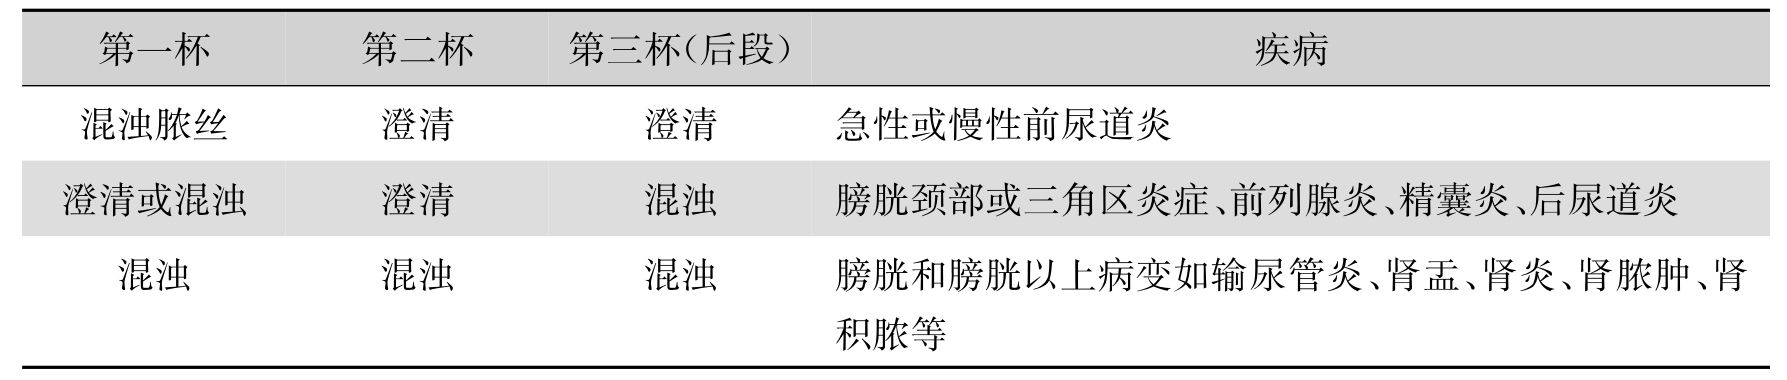
\includegraphics[width=5.94792in,height=1.25in]{./images/Image00229.jpg}
\end{table}

\subsubsection{2.脓尿伴随的症状}

\paragraph{(1)疼痛:}

脓尿伴有肾绞痛者,多提示病变位于肾脏,如肾结石合并感染、肾结核、肾积脓、肾脓肿、丝虫乳糜脓尿等;如伴有膀胱区痛者,则提示病变已侵及膀胱,如泌尿系结核。膀胱结石或感染,膀胱邻近器官脓肿如阑尾周围脓肿、盆腔脓肿等向膀胱穿破;如伴有尿道烧灼痛,则提示病变已侵犯尿道、前列腺,如尿道炎、前列腺炎等。

\paragraph{(2)膀胱刺激征(如尿频、尿急、尿痛等):}

上尿路感染在未侵犯膀胱之前或脓液不多,一般无膀胱刺激征或症状较轻;下尿路感染则此症状较严重。

\paragraph{(3)痛性肿块:}

如肿块位于肾区,应考虑肾脓肿、肾积脓、肾周围脓肿、肾肿瘤等;如肿块位于膀胱区,则应考虑巨大膀胱憩室或肿瘤;如肿块位于右(左)下腹部,应考虑阑尾周围脓肿,输卵管、卵巢脓肿等。如肾区同时伴有局部皮肤红、肿、热者,则多为肾周脓肿或肾周围蜂窝织炎。

\subsubsection{3.实验室检查}

尿常规检查,尿中含有轻度蛋白质或各种管型,尤其是白细胞管型者,则病变多位于肾脏,如肾盂肾炎等。白细胞酯酶试验可检测尿白细胞,亚硝酸盐试验对革兰氏阴性细菌诊断较敏感。此外,也可作尿Tamm-Horsfall蛋白包裹游离细胞检测(用荧光标记的抗人Tamm-Horsfall蛋白抗体检查尿中的游离细胞),如为阳性(>12\%),则有助于肾实质性疾病的定位诊断。相反。如尿中蛋白质及管型阴性,则以肾脏以下部位的感染的可能性大。如脓尿中含有较多的红细胞,则应考虑肾结石、肾盂肾炎、肾结核或肾肿瘤合并感染等可能。

如脓尿中含有乳糜尿则考虑丝虫病所致。此外,尿沉渣涂片找菌及寄生虫或虫卵(如微丝蚴、滴虫、血吸虫、包虫等),或尿培养等,对确定病原也有重要意义。

如对尿路细菌感染的部位不能确定是上尿路抑或下尿路感染时,可作以下检查:

①消毒膀胱后取尿作细菌培养或经膀胱镜插入输尿管收集肾盂尿作细菌培养,此法较复杂,对患者有一定的痛苦。②尿液抗体包裹细菌(antibody
coated
bacteria)检查,应用荧光标记的免疫球蛋白处理尿沉淀中的致病细菌,如发现细菌有荧光抗体包裹,则可确定为肾盂肾炎,阴性则为膀胱炎。但必须注意,慢性前列腺炎时尿中也可发现抗体包裹细菌。

如多次常规尿培养为阴性(能排除其他因素影响),呈“无菌性脓尿”,且尿经常呈酸性者,则应考虑泌尿系结核,作细致的尿结核杆菌检查。

肾功能检查:对肾盂肾炎和膀胱炎有一定鉴别诊断意义。如发现有尿浓缩功能或酚红排泄功能降低者,则多为肾盂肾炎而非膀胱炎。

\subsubsection{4.特殊检查}

根据上述临床表现及一般实验室检查,对脓尿的病变部位及性质常可作出比较正确的初步判断。如诊断尚未明确,则可有目的、有步骤地选用有关特殊检查,如膀胱镜检查、X线腹部平片及尿路造影术、超声波、放射性核素肾图或CT、MRI等检查,此类检查对确定病变部位及性质均有一定的诊断价值。

临床上能引起脓尿的疾病较多(表\ref{tab36-7})。大致可分为:①泌尿系统疾病(包括上尿路和下尿路疾病);②生殖系统疾病;③泌尿生殖系统邻近器官或组织疾病等三大类。现分述于下。

\begin{table}[htbp]
\centering
\caption{脓尿疾病的分类}
\label{tab36-7}
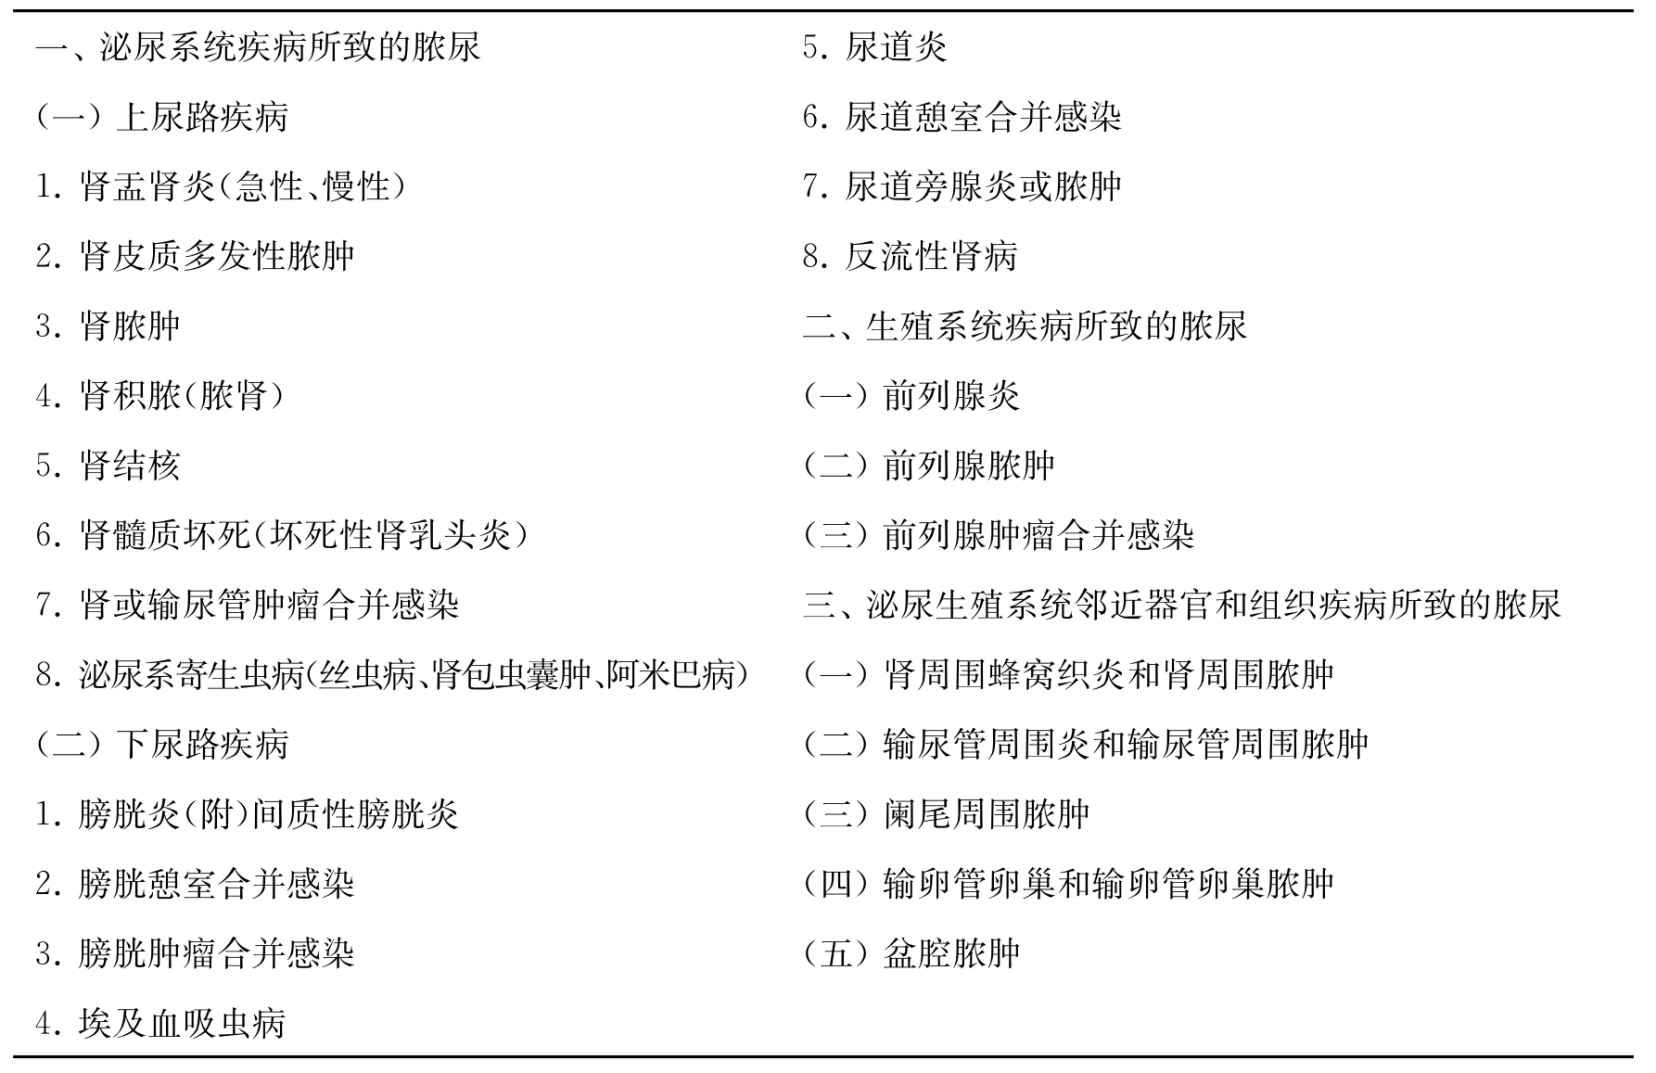
\includegraphics[width=5.94792in,height=3.84375in]{./images/Image00230.jpg}
\end{table}

\protect\hypertarget{text00283.html}{}{}

\subsection{121.1 泌尿系统疾病}

\subsubsection{121.1.1 上尿路疾病}

\paragraph{一、肾盂肾炎}

肾盂肾炎为常见的泌尿系感染性疾病。多见于生育期女性,尤其多发生于妊娠或产褥期,婴幼儿患者也不少。各种能引起尿路梗阻和尿液滞留的疾病。如结石、妊娠子宫压迫输尿管、前列腺肥大、肾下垂、游走肾、肿瘤、糖尿病等,是常见的诱因。尸检资料证明,有尿路梗阻较无梗阻者肾盂肾炎发病率高12倍。瘫痪患者和泌尿道畸形患者也较易患此病,手术及器械操作如导尿(特别是停留尿管)、膀胱镜检查之后也易引起感染。病原菌绝大多数为大肠杆菌,其次为葡萄球菌、副大肠杆菌、粪链球菌、变形杆菌、铜绿假单胞菌、产气杆菌等。

临床上分为急性和慢性两种:

\subparagraph{(一)急性肾盂肾炎}

急性肾盂肾炎是指病程不超过六个月者。其典型的临床表现为:①急起畏寒、发热;②有明显的腰酸痛、尿频、尿急、尿痛等尿路刺激症状;③明显肾区压痛及叩击痛;④不同程度的脓尿(可有白细胞管型),轻度蛋白尿约+~++(不超过1g/24h);⑤尿培养细菌阳性。

脓尿是本病诊断的关键,几乎全部患者均有不同程度的脓尿,但多数为镜下脓尿(白细胞多为+++~++++),结合临床表现一般即可确诊。有时在血行性感染性肾盂肾炎早期,常以发冷、发热等全身感染症状为主要表现,而泌尿系统感染症状不明显甚至缺乏时,如不注意尿液的检查,常被误诊为流感、疟疾、伤寒、大叶性肺炎或“发热待查”等;有的患者因有血尿、肾绞痛而被误诊为肾结石或肾结核;有的患者因恶心、呕吐、腹泻而被误诊为急性胃肠炎(尤其小儿患者更常见);也有以急性腹痛为主诉而误诊为急性阑尾炎或急性胆囊炎者。因此,最主要的鉴别方法为反复做尿沉渣检查,镜下脓尿为重要的鉴别根据之一。

急性肾盂肾炎常与单纯性急性膀胱炎相似,两者虽均有脓尿,但后者以耻骨上腹痛及压痛为主,而无腰痛和肾区叩压痛,膀胱刺激症状明显,较多出现终末血尿,一般无发热(小儿除外),也无管型尿和蛋白尿等。

\subparagraph{(二)慢性肾盂肾炎}

慢性肾盂肾炎系指症状迁延不愈,病程超过六个月以上者;或者病程不明确,但在肾盂肾炎症状控制后仍有肾功能不全或肾盂造影有X线异常表现者,也为慢性肾盂肾炎。本病通常由急性肾盂肾炎发展而来,但也有为潜行性而无明显的急性期症状。慢性肾盂肾炎发作期有较明显的全身与泌尿系统感染症状,而在间歇期中则往往以腰部隐痛、多尿(特别在夜间)及轻度脓尿为最常见的三项症状。诊断慢性肾盂肾炎的主要根据为:①半年以上反复发作的急性肾盂肾炎病史,或腰痛、尿频与脓尿史;②现有不同程度的腰痛、尿频、肾区叩击痛等泌尿系病征;③尿培养细菌阳性,或培养虽为阴性,而尿沉渣内白细胞增多始终存在,并除外其他泌尿系疾病者;④病程不明确,但已有不同程度的肾功能减退(尤以浓缩功能、酚红排泌功能)者。如有上述的典型表现,诊断一般较易。临床上常表现有典型和不典型两类。典型者有反复发作泌尿道感染症状,尿改变明显,间可出现肉眼血尿,而肾功能损害较少,称为慢性泌尿道感染型肾盂肾炎。不典型者常缺乏明显泌尿道症状,其中有部分患者呈慢性潜行性经过,无特殊不适,尿改变极轻,而持续有细菌尿,称为潜隐型慢性肾盂肾炎;又有部分患者常有原因未明的长期低热,腰痛,疲乏,消瘦,贫血,以后逐渐出现肾衰竭;此外,也可发生恶性高血压,出现早期心、肾功能障碍及眼底改变,称为慢性肾内感染型肾盂肾炎。因此,对各类型的慢性肾盂肾炎的诊断要加以注意。

黄色肉芽肿性肾盂肾炎是慢性肾盂肾炎的一种罕见的类型,常见于中老年人,多累及一侧肾。临床表现为反复尿感发作,肾区疼痛,发热、消瘦、贫血、体重下降、腰痛、伴腹部肿块。该病与肾结核临床表现及声像图极为相似,需加以鉴别。B超声和X线显示肾体积增大,形态失常,肾内多个低回声区合,伴钙化、梗阻。对于有反复发作脓、血尿迁延不愈,肾脏增大伴有积液的患者,应考虑本病的可能,及时做B超和X线影像学复查并与肾结核仔细鉴别。由于本病超声图像缺乏特异性,与肾结核弥漫型极为相似,必要时应做晨尿检查寻找泡沫细胞或超声引导下肾脏穿刺活检,本病常需病理检查才得以确诊。病变特征为肾实质破坏,有肉芽肿,脓肿和泡沫细胞。确诊有赖于CT,MRI和病理检查。

我院总结的297例肾盂肾炎中。呈典型反复发作泌尿道症状者仅为2/3左右,不典型表现者有:①呈“潜隐型”表现者约占17.7\%;②以反复发作寒热而无泌尿系症状类似感冒、疟疾、伤寒者约占3\%;③有以血尿为主要表现,易误诊为肾结石或肾结核者占3\%;④有以急腹痛为主要表现而误诊为急性阑尾炎或胆囊炎者约占1.3\%;⑤有以肾绞痛为主要表现而误诊为肾结石者约占2\%;⑥有病程缓慢,缺乏明显症状,而出现明显高血压或尿毒症症状方初次就诊者约占2.4\%;⑦有暴发类型而死于败血症或急性肾功能不全者约占1.3\%。据文献报道,肾盂肾炎除有上述不典型表现外,还可有高血压脑病、左心衰竭、类白血病反应和肾小管功能障碍等临床表现。

由于有些慢性肾盂肾炎的临床表现不典型,因此实验室检查对诊断极为重要。分述于下:

\hypertarget{text00283.htmlux5cux23CHP36-4-3-1-1-2-1}{}
1.尿常规检查

脓尿是诊断慢性肾盂肾炎的重要病征。其特点多为小量的镜下脓尿,常为+~++,间歇出现。有人认为,如尿沉渣检查发现白细胞每高倍视野5个或5个以上者提示为脓尿,但少于5个白细胞时却不能除外脓尿;未经离心沉淀的新鲜尿液中,如每高倍视野超过3个者,即可诊断为病理性白细胞尿,表示有泌尿系感染,可提供临床参考。由于肾盂肾炎患者的脓尿可间歇出现,因此,对可疑病例,不能只检查1~2次尿,而应反复多次检查新鲜晨尿。

\hypertarget{text00283.htmlux5cux23CHP36-4-3-1-1-2-2}{}
2.每小时尿白细胞排泄率的测定

此测定对慢性肾盂肾炎的诊断有较大的意义,尤其对普通尿沉渣检查无白细胞增多者更有价值。正常人每小时尿内白细胞数在20万个以下(近来国内有人认为男性正常值<7万/h,女性在<14万/h);20万~40万个之间为可疑:40万个以上者,则慢性肾盂肾炎的可能性极大。阳性率可高达91.7\%。由于本病常以间歇性脓尿为特征,怀疑病例如尿液中无肯定阳性结果时,应再次复查。如多次检查均在正常范围内,而临床又有尿路感染的依据,可考虑作肾上腺皮质激素尿白细胞排泄率测定。但要注意,本试验副作用较多,不能作为常规检多项目,有镜下血尿者不宜施行。

\hypertarget{text00283.htmlux5cux23CHP36-4-3-1-1-2-3}{}
3.12小时尿细胞计数(Addis计数)

对常规尿沉渣检查阴性的患者有协助诊断价值。如发现白细胞增多远较红细胞增多明显,且白细胞总数超过100万个时,则有助于慢性肾盂肾炎的诊断,可借此与慢性肾炎或高血压性肾病鉴别。

\hypertarget{text00283.htmlux5cux23CHP36-4-3-1-1-2-4}{}
4.尿细菌学检查

对慢性肾盂肾炎的诊断及治疗均有决定性意义,尤其对无症状、尿沉渣检查无白细胞或白细胞不多、仅有菌尿症的潜隐型慢性肾盂肾炎更为重要。一般可采用普通尿沉渣涂片染色检菌,或不染色直接找菌,中段尿培养和尿定量培养等方法。

\hypertarget{text00283.htmlux5cux23CHP36-4-3-1-1-2-4-1}{}
(1)清洁尿普通涂片染色检菌或不染色直接找菌:

此法简便,在设备条件差的医疗单位可以采用,阳性率可高达92.6\%,不但可找到细菌而且还可确定致病菌是杆菌或球菌,革兰氏染色还可分别为阳性菌或阴性菌。检菌阳性常示患者有活动性肾盂肾炎。

\hypertarget{text00283.htmlux5cux23CHP36-4-3-1-1-2-4-2}{}
(2)中段尿培养:

可确定病原,但一次培养阴性不能排除本病的存在。

\hypertarget{text00283.htmlux5cux23CHP36-4-3-1-1-2-4-3}{}
(3)细菌定量培养:

是最确定的诊断方法,据一般报告,中段尿定量培养每毫升尿中细菌数在10万个或更多时,可诊断为真性细菌尿;1万~10万之间为可疑,如同时并有明显症状时,仍有诊断价值,应复查;在1万个以下则感染的可能很小,在1000个以下则多为污染。对繁殖力低的细菌如肠球菌、粪链球菌等,如每毫升尿中细菌数达5000个者也有诊断意义。但须注意:在抗菌药物治疗期间或停药后不久,尿液因补液、利尿而稀释。尿在膀胱停留期间过短或因输尿管引流受阻以致肾盂尿进入膀胱的量过少,尿pH值过低或过高等因素,均可使细菌定量培养呈假阴性。此外,有部分尚未表现临床症状的肾盂肾炎患者尿细菌数可不高。故对此结果应密切结合临床具体情况,作全面的诊断分析。

\hypertarget{text00283.htmlux5cux23CHP36-4-3-1-1-2-5}{}
5.亚硝酸盐还原试验(Griess试验)

此试验简便、迅速,在缺乏尿培养条件的情况下对肾盂肾炎的诊断有以下帮助。此试验一般不发生假阳性,因此,当检查得到阳性结果时,大致可肯定肾盂肾炎的诊断,但阴性不能排除泌尿道感染的存在。对大肠杆菌、副大肠杆菌、肺炎杆菌、变形杆菌等所致的泌尿道感染阳性率高;对葡萄球菌、产气杆菌及铜绿假单胞菌则阳性率较低;对结核杆菌、链球菌、淋病双球菌、肠炎杆菌属及其他革兰氏阴性菌均呈阴性反应。因此,本试验除可应用作诊断泌尿道感染的方法外,还对单纯肾结核与慢性肾盂肾炎有鉴别诊断意义。但要注意,在抗菌治疗后,或在利尿过程中,或患者有尿频、尿急。尿液停留在膀胱内的时间短,因尿中含亚硝酸钠量少可导致阴性反应。

\hypertarget{text00283.htmlux5cux23CHP36-4-3-1-1-2-6}{}
6.白细胞酯酶试验

该方法可检测出25~50个白细胞/毫升,目前,临床用的快速浸渍试纸就是利用亚硝酸盐还原和白细胞酯酶试验结合而成,具有快速筛选尿感作用。

\hypertarget{text00283.htmlux5cux23CHP36-4-3-1-1-2-7}{}
7.尿液抗体包裹细菌检查

阳性可确定为肾盂肾炎,阴性为膀胱炎,但注意前列腺炎时也可呈阳性。

在一般病例中,根据病史、症状、尿沉渣检查及尿培养细菌阳性即可作出诊断。对不典型病例,则应提高本病诊断的警惕性,需结合各种实验室检查资料进行诊断。在少数诊断较困难或久治无效的患者,应作B超、X线腹部平片检查是否合并泌尿系结石,或进一步作静脉肾盂造影,如发现肾盏呈杵状,或轻度的肾盂肾扩张,或肾盂、肾盏轮廓不规则、瘢痕性畸形等,对诊断有一定帮助;此外,也可发现久治无效的影响因素,如先天性肾或肾盂、输尿管异常,肾下垂或游走肾,肾积水,进X线的肾结石,肾结核或肾肿瘤等病理状态等,对指导治疗也有重要价值。对极少数与其他肾脏疾病难以区别的病例,可作CT、MRI、血管造影等检查,必要时可作肾穿刺活体组织检查以助诊断(表\ref{tab36-8})。

\begin{table}[htbp]
\centering
\caption{慢性肾盂肾炎和慢性肾炎的鉴别诊断}
\label{tab36-8}
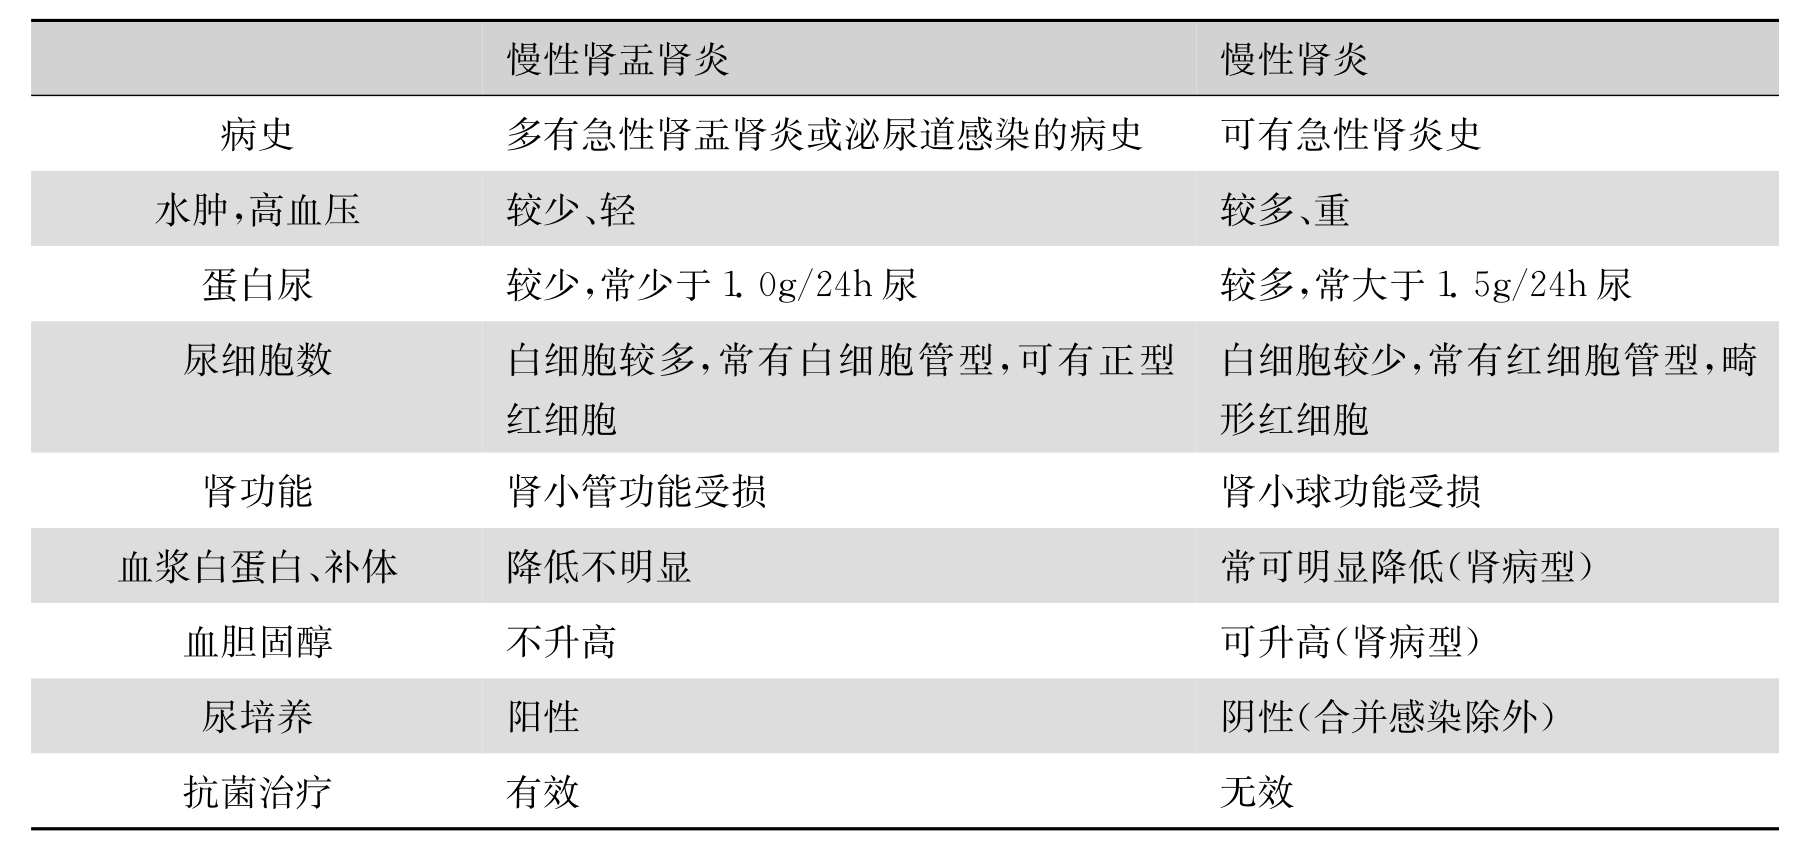
\includegraphics[width=5.98958in,height=2.82292in]{./images/Image00231.jpg}
\end{table}

慢性肾盂肾炎以血尿为主要临床表现时,常需与肾结石,肾结核相区别;此外,慢性肾盂肾炎无明显泌尿系症状,以高血压、尿毒症为主要临床表现时,常与慢性肾炎相混淆,两者治疗与预后均有很大的不同,故鉴别诊断很重要。其鉴别要点参见表\ref{tab36-6}。潜隐型慢性肾盂肾炎常与隐匿型慢性肾炎相混淆,从多次尿常规检查可发现前者以白细胞为主,而后者有较多的红细胞,或有红细胞管型;此外,观察患者有否低热、尿频等症状,尿培养有无细菌等也有助于鉴别。

慢性肾盂肾炎需与单纯慢性膀胱炎及慢性前列腺炎相鉴别。后两者有脓尿而无管型尿,无蛋白尿,尿三杯试验时白细胞在第三杯最多,尿抗体包裹细菌检查阴性,也无肾功能减退的表现。如患者有脓尿、排尿痛及终末血尿,支持慢性膀胱炎的诊断。慢性前列腺炎时,尿道口每有黏性脓性分泌物,前列腺触诊腺体肿大而有压痛,腺体的全部或局部变硬,按摩后尿道口常有分泌物流出(前列腺液),呈黏液脓性,镜检可发现白细胞增多超过10个/高倍视野,磷脂酰胆碱小体明显减少,干后染色或可找到细菌。慢性肾盂肾炎有时产生急进型高血压的表现,此时需与急进型高血压相鉴别。慢性肾盂肾炎发病年龄较轻,肾功能损害每于反复感染后加重,肾功能损害较重(肾小球滤过率低于30ml/min,尿比重低于1.012,且固定),12小时尿细胞计数有白细胞与红细胞分离现象(白细胞较红细胞显著增多)。

\subparagraph{(三)老年性肾盂肾炎}

老年人随着年龄增长,逐渐出现器官萎缩和功能减退,全身免疫功能减退,和泌尿生殖系统的局部免疫能力下降,抗病能力下降,容易导致感染,其中尿路感染即是其中常见病之一。老年人肾盂肾炎的临床特点,老年人肾盂肾炎患者约1/3无临床症状,无尿路刺激征,可仅表现无症状性菌尿、常在代谢性疾病,尿路不通畅等易感因素下诱发尿感,治疗效果也不佳。因此,临床上对于伴有糖尿病、前列腺疾病、尿路结石、近期导尿或留置导尿管或作过尿路检查、曾长期使用激素或免疫抑制剂以及习惯性便秘者应多加注意。及时送尿沉渣镜检,脓尿有助于诊断,但清洁中段尿培养对确定老年人尿路感染非常重要,必要时超声波、IVP、CT和MRI等检查。

\paragraph{二、反流性肾病(RN)又称膀胱输尿管反流}

反流性肾病是指膀胱输尿管反流导致肾瘢痕形成、缓慢发展而成的终末期肾脏病。临床上常有反复发作性尿感,伴膀胱刺激征,严重者有急性肾盂肾炎,如患者临床上有反复尿感,肾瘢痕或单则肾萎缩常常需考虑排除此病。成人患者还可有蛋白尿、高血压、夜尿、多尿、肾衰竭等症状。妊娠期高血压可为首发症状,并加重肾脏损害。诊断依靠排尿期膀胱尿路造影、放射性核素、静脉肾盂造影、超声波和膀胱镜。膀胱输尿管反流(VUR)诊断时,超声检查可作为筛选方法。尤以彩色多普勒检测。排尿性膀胱输尿管造影是重要的诊断手段,但敏感性较低。放射性核素检查有较高的敏感性,间接法还较直接法方便,还适用于尿路感染急性期。国内报道一组65例中,曾对一批慢性尿路感染患者作静脉肾盂造影加断层扫描、肾脏CT、MRI、排尿性膀胱肾盂造影、核素间接法膀胱造影等,检查发现肾盂变形,肾发育停滞,输尿管、肾盂扩张,不同程度的膀胱输尿管反流等改变,据此作出反流性肾病的诊断。

\paragraph{三、肾结核}

凡有明显尿频、尿急、尿痛等膀胱刺激征,如反复发作,抗菌治疗不佳或尿培养无细菌生长,均要考虑肾结核的可能。肾结核病尿呈酸性,几乎都有不同程度的脓尿,早期仅于镜下发现少量白细胞及红细胞,后期如发展为结核性肾积脓时,则尿中可出现干酪样物质,使尿呈米汤样混浊。肾结核常伴肾外结核如肺、附睾结核等,诊断需尿沉渣找抗酸杆菌、结核菌培养、静脉肾盂造影和膀胱镜检查来确诊。静脉肾盂造影显示肾乳头坏死、肾盂虫蚀状、空洞或肾盂完全不显影、输尿管僵直、虫蚀样边缘、管腔狭窄、有时可见钙化。肾结核表现为膀胱刺激征和血尿时常需与非特异性膀胱炎、结石和肿瘤等进行鉴别诊断。非特异性膀胱炎常突然发生,并可反复发作,时轻时重,血尿常与膀胱刺激症状同时发生,一般抗感染治疗效果较好。而肾结核引起的结核性膀胱炎以尿频开始,逐渐并持续加剧,而不呈间歇性发作,血尿都在膀胱刺激症状一段时间后才出现。但在结核性膀胱炎合并非特异性感染时,则需通过细菌学检查才能鉴别和确诊。此外,膀胱尿道梗阻性病变引起的尿频、尿急、尿痛均在排尿困难症状以后发生,多数伴有非特异性感染。膀胱结石的膀胱炎在排尿时可有尿线突然中断,伴有尿道内剧烈疼痛。膀胱肿瘤的膀胱刺激症状都在长期无痛血尿以后才出现,此时肿瘤已有浸润或邻近三角区,而肾结核血尿多在长时间尿频以后,以终末血尿为其特点(参见第1节)。

\paragraph{四、肾皮质多发性脓肿}

此病实际是血行性感染性肾盂肾炎。病变多为双侧性、肾皮质多发性小脓肿,也可侵犯肾髓质,如病变继续发展,小脓肿可互相融合、扩大而形成肾脓肿或肾痛。本病多继发于皮肤化脓性感染或上呼吸道感染,细菌经血道而感染肾脏。致病菌大多数为金黄色葡萄球菌。其临床特点与急性肾盂肾炎稍有不同,有持续高热、寒战、白细胞增高等菌血症表现,但无膀胱刺激征,有较明显腰痛、腰肌痉挛及肾区压痛和叩击痛;早期一般无脓尿,但当病变侵犯肾小管时,才发现镜下脓尿。尿沉渣涂片染色检查及(或)尿培养可发现葡萄球菌。如有上述典型的表现,即可成立。有时由于无明显泌尿系症状和脓尿,部分呈脓尿,尤其部分呈亚急性或慢性过程的患者,临床表现不典型而导致延误诊。故在临床上,如患者有化脓感染的原发病史,突然高热、寒战,同时伴有腰痛及明显肾区压痛和叩击痛,尿中有镜下脓尿者,即应考虑本病的可能,但需除外肾周围蜂窝织炎及肾周围脓肿。此外,本病常与腹腔器官(如胆囊、阑尾等)后腹膜的急性感染疾病相混淆,尿沉渣中白细胞增多和涂片染色中尿培养检菌是其重要的鉴别方法。

\paragraph{五、肾脓肿}

肾脓肿是由肾皮质多发性脓肿发展、融合扩大而成。如肾脓肿向肾盂穿破时即可引起明显肉眼脓尿,但临床上较少见;向肾周围渗出形成肾周围脓肿尿,由于尿路受脓液刺激或继发感染,可出现膀胱刺激症状,与此同时,因脓液向肾盂引流,腰痛可显著缓解,肾压痛及叩击痛也相应减轻。较大肾脓肿超声波检查可协助诊断。静脉肾盂造影见肾盂、肾盏变形或充盈缺损等征象,也有助于诊断。

\paragraph{六、肾积脓(脓肾)}

肾积脓是一种极严重的肾化脓感染,多并发于肾结核、肾结石、肾盂肾炎及肾积水合并感染等疾病。脓尿是其突出的表现,在输尿管与脓肾相通时,可出现持续大量肉眼脓尿。如果输尿管因脓肿或炎性瘢痕、水肿、痉挛而引起阻塞时,则脓尿可不明显或消失,也可呈间歇性脓尿。此外,本病发病过程有急、有慢,临床表现也有不同。如为急性感染引起者,除有全身感染中毒症状外,还有明显的局部症状,如腰痛、腰肌紧张、肾区明显压痛及叩击痛等,腹部检查可触及肿大的肾脏;如为慢性感染引起者,则呈慢性感染中毒现象,如微热、盗汗、消瘦、贫血等,局部症状较轻。上述的临床表现,一般诊断不难。肾超声检查对较大肾积脓有一定诊断意义。放射性核素肾图检查也有诊断价值。静脉肾盂造影,可见患肾不显影,表示肾功能丧失,也有助于诊断。

由于肾积脓的原发疾病的治疗和预后均有很大的不同,故原发病的鉴别诊断更为重要。如肾结核合并感染所致的脓肾,多为慢性过程,多有其他器官结核病,如肺结核、附睾结核等,脓尿中有干酪样物质,呈米汤样混浊,尿中有大量结核杆菌。肾结石继发感染引起的脓肾,多有反复肾绞痛、血尿病史。肾盂肾炎引起脓肾,多由于严重血行性感染性肾盂肾炎、肾皮质多发性脓肿侵犯肾盂所致,多呈急性过程,有明显全身性菌血症症状。肾积水继发感染所致的脓肾,多有肾结石或肾结核、或其他尿路阻塞的病史,腹部可摸到肿大的肾脏。

\paragraph{七、肾髓质坏死(坏死性肾乳头炎)}

本病是肾盂肾炎的严重并发症。病势凶险,症状严重,死亡率很高,故有人称之为“暴发型肾盂肾炎”。本病较少见,多发生于40岁以上,约有57\%患者并发于糖尿病。尿路梗阻也为重要的诱发因素(如前列腺肥大、输尿管梗阻、先天尿路畸形等),其他肾脏病变如肾血管病变等也可并发此病。国外文献报道,大量长期服用镇痛剂如非那西丁等可直接损害肾脏,故称为“镇痛药性肾病”,当其发生继发感染时可产生本病;其病理解剖特点多为双侧性及广泛性肾乳头炎症、化脓、坏死,且肾实质也有小脓肿形成。偶也可见单侧性或局限性病变。

临床上多数患者起病急骤,虽重型肾盂肾炎的临床表现,腰剧痛,大量脓尿、蛋白尿、管型尿及不同程度血尿,尿培养细菌阳性,尿中有时可见有坏死脱落的肾乳头组织块,严重者可发生少尿或无尿,进一步出现尿毒症、酸中毒,甚至引起昏迷及休克等危险现象。部分患者可呈亚急性经过,病程稍长,数周至数月,感染症状较轻,但常有进行性肾功能减退,有时因坏死乳头脱落阻塞输尿管而致肾绞痛,与肾结石相类似。

此外还有少数患者呈慢性经过(多见于“镇痛药性肾病”患者),病程可达数年,临床表现类似慢性肾盂肾炎,各种症状可间歇出现,或无任何症状,以后逐渐出现肾功能减退。

在临床上由于本病病情危重,早期诊治甚为重要,根据上述典型表现,结合患者原发病病史,发现尿中脱落的坏死乳头组织块等,即应考虑此病存在的可能。静脉肾盂造影有助于诊断。

\paragraph{八、肾或输尿管肿瘤合并感染}

肾、输尿管肿胀引起尿路梗阻或因肿瘤本身溃烂、坏死,容易合并细菌感染而出现不同程度的脓尿。但这些患者起初常以血尿为主,其临床特征参见第119.1.4节。

\paragraph{九、泌尿系寄生虫病}

\subparagraph{(一)丝虫病}

当丝虫病引起乳糜尿时,乳糜可刺激尿路或引起尿路梗阻,常合并感染而出现乳糜脓尿(参见第122节)。

\subparagraph{(二)肾包虫囊肿}

本病少见,国内仅有少数病例报告,多伴有身体其他脏器包虫囊肿。肾包虫囊肿向肾盂穿破或继发感染时,可出现脓尿及膀胱刺激症状。其主要特征为腹部检查可触及肿大的肾脏,偶尔尿中发现包囊虫卵即可确诊。一般病例结合流行史、皮内抗原试验、超声波、X线腹部平片及肾盂造影检查等可明确诊断。根据上述情况并可与肾单纯囊肿、多囊肾及肾积水并发感染相区别。

\subparagraph{(三)泌尿系阿米巴病}

患者有阿米巴痢疾史,出现发热、腰痛、膀胱刺激征,尿呈果酱色,镜检大量脓细胞,并有阿米巴滋养体。

\subsubsection{121.1.2 下尿路疾病}

\paragraph{一、膀胱炎}

膀胱炎几乎全为继发性。可继发于泌尿系疾病,如肾感染、尿道感染、结石、结核、肿瘤等,也可继发于泌尿系外的疾病,如生殖器官炎症、神经系疾病、胃肠道疾病等。女性较多见。急性期可有明显肉眼脓尿,膀胱刺激症状显著,但一般无发热;慢性期症状较轻,但反复发作。

对慢性反复发作、经久不愈的慢性膀胱炎患者,应仔细找寻原发病因。慢性膀胱炎常继发于肾盂肾炎、肾结核、前列腺炎、泌尿系结石等疾病。

\subparagraph{附:间质性膀胱炎}

本病国内少见,多见于成年女性,病因未明。临床表现与普通膀胱炎相似,其所不同者为;①间质性膀胱炎除于排尿和排尿终末时有疼痛外,于膀胱胀满时疼痛更剧;②患者虽有明显膀胱刺激症状,但尿中很少有炎性成分,甚至无白细胞或脓细胞;③尿培养细菌阴性;④膀胱镜检查见膀胱容量缩小,溃疡病变多见于膀胱圆顶及前壁。

\paragraph{二、膀胱憩室合并感染}

膀胱憩室一般无症状,如合并感染时可出现脓尿及膀胱刺激症状。少数患者可因感染产生炎症溃疡而出现血尿。部分患者可有“二段排尿”现象。膀胱镜或膀胱造影检查可确诊。

\paragraph{三、膀胱肿瘤合并感染}

当膀胱肿瘤产生溃疡或引起尿路梗阻时,常并发尿路感染而产生脓尿。主要的临床表现为血尿及膀胱刺激症状。

\paragraph{四、埃及血吸虫病}

本病主要侵犯膀胱,其次为输尿管下段。当炎症病变发生溃疡或合并细菌感染时可出现明显脓尿。其主要表现为血尿、膀胱刺激症状及尿中找到埃及血吸虫卵。国内未见有此病报告。

\paragraph{五、尿道炎}

尿道炎很常见,以大肠杆菌、链球菌和葡萄球菌所致的尿道炎为最常见。目前,淋病双球菌、支原体衣原体、所致尿道炎逐渐很多。

女性尿道炎非常常见。由于女性尿道短而直,常向上侵犯膀胱,易受肛门肠道感染故称之为“女性肠尿道炎”。常为蛲虫病和阴道滴虫病的并发症,小儿尿道远端梗阻、膀胱颈梗阻、后尿道瓣膜等解剖异常可诱发本病;成年妇女多于新婚期或生育期发病;常为尿道周围腺感染所引起;绝经期后的老年性尿道炎,则为雌激素活性降低、尿道黏膜萎缩所致。发病多为急性,也可呈慢性反复急性发作。其主要特点为:脓尿与显著的膀胱刺激症状,如尿频、尿急、尿痛等,严重者可出现血尿。临床上常误诊为肾盂肾炎,但本病一般无发热,很少有腰痛,肾功能正常。此外,部分慢性发作、经久不愈的患者,常需与泌尿系结核、膀胱结石或肿瘤等相区别,可作尿液结核菌检查、腹部X线平片、肾盂造影和膀胱镜检查等以排除。

男性尿道炎的临床表现也以脓尿、膀胱刺激征和尿道压痛为特点,可分为前尿道炎和后尿道炎。后尿道炎与前列腺炎常同时并存。采用尿三杯试验有助于前、后尿道炎的鉴别诊断。

由于男性慢性尿道炎多与各种原因的尿道梗阻,泌尿生殖系其他部分或其邻近器官炎症等同时并存,故在临床上,不要满足于单纯慢性尿道炎的诊断;必要时,还需作前列腺检查及膀胱尿道镜检查等进一步明确诊断。尿道脓性分泌物的细菌及寄生虫检查,对确定病因及治疗也有重要意义。

\paragraph{六、尿道憩室合并感染}

尿道憩室女性多见。临床表现与慢性尿道炎和膀胱炎相似,如尿频、尿急、尿痛、尿潴留、血尿、脓尿等,阴道检查于阴道前壁可触及一软性肿块,局部有压痛,可挤出脓液。尿道镜检查及尿道造影术有助于诊断。

\paragraph{七、尿道旁腺炎或脓肿}

女性尿道旁腺炎症或脓肿形成,均可由腺管排出脓液而成脓尿。症状与尿道炎相似。注意尿道口两侧尿道旁腺的检查,一般较易诊断。

\protect\hypertarget{text00284.html}{}{}

\subsection{121.2 生殖系统疾病}

\subsubsection{一、前列腺炎}

此病是成人男性较常见的疾病。绝大多数是由于前列腺长期充血、腺泡淤积、腺管水肿所致;少数患者也可由细菌感染所引起。本病多呈慢性经过,但也有急性发作者。在急性发作时可出现脓尿,甚至出现终末血尿,常伴有畏寒、发热。如炎症累及尿道或膀胱三角区时,则出现明显膀胱刺激症状如尿频、尿急、尿痛等,而误诊为肾盂肾炎、肾结核、输尿管或膀胱结石、膀胱肿瘤等;此外,常伴有会阴部、腰骨部及直肠内肿痛(大便时加剧);如并发精囊炎时,有时可因邻近器官伴发感染引起腹部疼痛需与急性阑尾炎、急性胆囊炎或肾绞痛等急性腹痛相鉴别;因此,在诊断时要注意区分。在慢性期,一般症状较轻,脓尿较少甚至尿完全正常,但常伴有不同程度的性功能异常和变态反应性疾病,如关节炎、神经炎、虹膜炎等。

前列腺炎的诊断,尿三杯试验有一定的帮助;此外,直肠指检和前列腺液检查有助确诊。直肠指检在急性期可扪及前列腺肿胀、压痛;在慢性期则腺体较硬,表面不规则。前列腺液检查:白细胞显著增加或成堆分布,而磷脂酰胆碱小体减少(正常前列腺液在每高倍视野下含白细胞少于10个,有多量磷脂酰胆碱小体)。借此,也可与肾盂肾炎、肾结核等鉴别,但前列腺炎常与泌尿系疾病同时并存,即使已确诊为前列腺炎,也不能排除其他泌尿系更重要的疾病,而延误治疗,必须加以注意。

\subsubsection{二、淋 病}

淋病是淋病双球菌通过不洁性交及其他性行为引起泌尿生殖道感染所导致的急性或慢性炎症性疾病,在“性传播病”中其发病率较高,近年发病率有升高趋势。好发于男性,有不洁性交史,常为淋球菌性尿道炎。初发时一般为前尿道炎,有明显的尿道刺激征,伴脓性分泌物从尿道流出。淋菌首先感染尿道外口,逐渐向前尿道黏膜蔓延,并发展至后尿道炎。机体在感染淋球菌后可产生局部免疫反应,中性粒细胞可大量吞噬淋球菌于细胞的胞浆内,大量的多核细胞的吞噬作用及细菌死亡释放内毒素,使尿道黏膜上皮发生多灶性坏死,形成大量黄绿色黏稠脓液外溢,2周后约60\%的患者病变继续向上逆行蔓延引起急性后尿道炎。后尿道脓液多时,会反流入膀胱与尿液混合使尿混浊出现大量脓细胞,而随尿排出。淋病的诊断主要依据病史、临床表现及实验室检查。实验室检查方法有直接涂片淋球菌检查、淋球菌培养和血清学检查等,血清学试验的敏感性、特异性较低,目前尚无可靠的血清学检查方法诊断淋病。淋球菌培养所需的营养条件、生长条件要求较高,一般较难培养出来。患者有脓性分泌物时,用脓性分泌物涂片,可检到革兰氏阴性双球菌。没有尿道分泌物,可用脓尿沉渣进行涂片检菌,如在尿沉渣涂片的中性粒细胞胞浆内检出革兰氏阴性双球菌。也有助于诊断。

\subsubsection{三、前列腺脓肿}

本病较少见,多数由急性前列腺炎恶化发展而来。临床上可出现大量脓尿,明显排尿异常症状,如尿频、尿急、尿痛、排尿困难与急性尿潴留等,以及显著的全身感染中毒症状。直肠指检发现前列腺肿胀、波动感、剧烈压痛,并有脓液被压出;必要时局部前列腺穿刺可抽出脓液,这对诊治均有实际意义。

\subsubsection{四、前列腺肿瘤合并感染}

前列腺肿瘤可并发感染而引起脓尿,本病特点参见相应章节。

\protect\hypertarget{text00285.html}{}{}

\subsection{121.3 泌尿生殖系统邻近器官和组织疾病}

\subsubsection{一、肾周围蜂窝织炎和肾周围脓肿}

肾周围蜂窝织炎和和周围脓肿可来自肾脏化脓感染(如肾皮质脓肿、肾积脓、肾盂肾炎等)直接的蔓延,也可来自肾外感染(如皮肤化脓病变、阑尾积脓、肝脓肿等)经血源或直接扩散。肾周围蜂窝织炎与肾周围脓肿的临床表现相似,但以肾周围脓肿为重。两者的临床特点为:①全身感染中毒症状如寒战、高热等,尤以肾周围脓肿为更显著;②患侧明显腰痛,腰肌紧张或强直,患侧肾区皮肤凹陷性水肿或红、肿、热及压痛和叩击痛,尤以肾周围脓肿更为严重;③患者向健侧弯腰时可引起剧痛,但向患侧弯腰时痛减轻,故患者腰椎常向患侧弯曲;④肾周围脓肿可于腰部或胁腹部触及痛性肿块。肾周围蜂窝织炎一般不引起尿改变,因常有肾感染,故尿中可有脓细胞,但临床表现远超出尿改变的程度。如肾周围脓肿向肾盂穿破时,则出现大量脓尿,而全身症状及局部表现可明显减轻,肿块很快缩小或消失。

对血行感染的早期,症状较轻,诊断较难,因此,对皮肤化脓性感染患者,如经过几天后突感全身发热、寒战,同时并有腹背肿痛者,应考虑本病的可能。对肾脏感染直接蔓延者,发现症状较原来加剧、肾区明显压痛者,也应考虑本病的可能。如出现大量肉眼脓尿时,则可能性更大,但应与肾脓肿相区别。X线腹部平片检查对肾周围脓肿的诊断很有价值。典型的X线征为:肾区显影增加,肾阴影及腰大肌阴影消失,腰椎向患侧弯曲,患侧膈肌上升或运动受限。借此可与肾脓肿或肾积脓相区别。

\subsubsection{二、输尿管周围炎和输尿管周围脓肿}

当输尿管周围炎和输尿管周围脓肿侵犯输尿管时可出现脓尿,但其为腹腔内局部炎症,应有局限性腹膜炎的表现。

\subsubsection{三、阑尾周围脓肿}

阑尾周围脓肿向右侧膀胱壁穿破时可出现大量脓尿。患者于出现脓尿之前,都有明显急性阑尾炎病史,右下腹剧痛,发热;体检右下腹肌痉挛,阑尾压痛点有明显压痛、反跳痛及可触及边缘较清楚的肿块。出现脓尿后,肿块往往较前缩小,而同时伴有明显膀胱刺激症状。

\subsubsection{四、输卵管卵巢炎和输卵管卵巢脓肿}

当输卵管、卵巢炎症累及膀胱壁或输卵管、卵巢脓肿向膀胱穿破时,可出现不同程度的脓尿,但临床上较少见;前者通常仅为镜下脓尿,后者常为突然出现的肉眼脓尿。右侧输卵管、卵巢脓肿于出现脓尿之前先有右下腹痛,同时伴以发热,右下腹明显压痛,需注意与急性阑尾炎区别。妇科检查:盆腔内有压痛,如有脓肿形成则于同侧摸到痛性肿块。如脓肿向膀胱穿破,肿块可明显缩小,脓尿刺激膀胱可引起膀胱刺激症状。

\subsubsection{五、盆腔脓肿}

盆腔脓肿向膀胱穿破时,可产生大量肉眼脓尿,但患者于出现脓尿之前,先有下腹痛、发热、耻骨上区域有明显压痛;妇科检查可于盆腔内触及肿块,特别在子宫直肠陷窝处,有波动感,明显压痛。如脓肿向膀胱穿破,脓肿常明显缩小,可伴有显著的膀胱刺激症状。

\protect\hypertarget{text00286.html}{}{}

\section{122 乳糜尿}

从肠道吸收的乳糜液(脂肪皂化后的液体)不能按正常淋巴道引流至血液,而逆流至泌尿系淋巴管中,以致该淋巴管内高压、曲张、破裂,乳糜液溢入尿中,使尿呈乳白色,临床上称此种尿为乳糜尿。

乳糜尿的混浊度及颜色可依乳糜含量的多少而异,而乳糜含量又常受患者的运动强度、食入脂肪量、淋巴管破裂程度等因素所影响。乳糜尿可呈乳白色、乳酪样或色泽稍混浊。其主要成分为磷脂酰胆碱、胆固醇、及少量纤维蛋白原和白蛋白等。此外,尚含有多少不等的血液;如含血液较多,呈粉红色,则为乳糜血尿。如合并泌尿系感染,可呈乳糜脓尿。

乳糜尿在体外容易凝结成白色透明胶状凝块。较严重的乳糜尿静置后可分3层:上层为脂肪;中层为乳白色成色泽较清的液体,常有小凝结块混悬于其中;下层为红色或粉红色的沉淀物,内含有红细胞及白细胞等。实验室鉴定:加乙醚于乳糜尿中,充分混合后,如能使尿液转澄清,即为乳糜尿。

乳糜尿应与脓尿、含多量盐类尿及脂肪尿相区别。脓尿于显微镜下可见大量脓细胞,临床上有泌尿生殖系感染表现;盐类尿于加热加酸后即转澄清;脂肪尿不含纤维蛋白原,无凝结现象,离心沉淀后脂肪浮于尿液的上层,镜检可见大量脂肪球,临床上常见于各种原因所致的肾病综合征,特别是类脂性肾病,其次亦可见于糖尿病肾病,狼疮性肾病,骨折,或砷、一氧化碳中毒,Fabry病等。

乳糜尿的发病机制目前尚无定论。文献中有些资料认为乳糜尿是由于胸导管及其支流阻塞所致,淋巴造影也有足够的资料阐明,也曾有作胸导管奇静脉吻合术治疗患者而获得颇为满意的疗效,故认为乳糜尿不是由于腹部淋巴道阻塞所致,乃因腹部淋巴管非常丰富;相互沟通形成淋巴管网,不易使乳糜的向上通道受阻而产生尿路淋巴瘘,但另一些资料却认为多数患者阻塞部位在胸导管之下。我院观感尿病例淋巴造影能显示胸导管者仅占少数。

一般地,乳糜尿的形成可有以下两方面的解释:

\subsection{一、广泛的腹部淋巴道阻塞}

正常从肠道吸收的乳糜液经肠干淋巴管达腹主动脉前淋巴结而至乳糜池。当腹主动脉前淋巴结或肠干淋巴管阻塞时,则乳糜液不能进入乳糜池,而通过腹主动脉前淋巴结与腹主动脉旁淋巴结之间的通路,流入腰干淋巴管而至乳糜池。如腰干淋巴管同时也有阻塞时,则乳糜液即逆流至泌尿系淋巴管,使其内压增高、曲张。终至破裂而产生乳糜尿。

\subsection{二、胸导管阻塞}

当胸导管下端阻塞时,则乳糜池内压增高,则乳糜液经腰干淋巴管反流至泌尿系淋巴管,使其内压不断增高,终至破裂而形成乳糜尿。

除上述淋巴道机械性阻塞的因素以外,淋巴管的先天异常(如淋巴管畸形及淋巴管瓣膜功能障碍等),也是产生乳糜尿的原因之一,但临床上极少见。

泌尿系淋巴管破裂的部位,最常见于肾盂(因肾脏的淋巴管最脆弱),其次为输尿管,有时也可见于膀胱、后尿道等处。

对于乳糜尿的诊断,应注意以下问题:

\subsubsection{(一)定位诊断}

乳糜尿的定位诊断包括乳糜液溢出部位和淋巴系阻塞病变部位两方面。在乳糜尿无特殊症状时,单凭临床表现以估计乳糜尿的来源较困难。当乳糜合并全程血尿或乳糜块经过输尿管而引起肾绞痛时,则可提示乳糜尿来自肾脏。至于来自单侧或双侧肾脏,则膀胱镜检查有一定的帮助。在间歇期,无乳糜尿时,膀胱镜检查意义不大。逆行肾盂造影术,如见有肾盂淋巴逆流现象,可能对乳糜液溢出的定位诊断有参考价值;但有人指出,正常逆行肾盂造影时也可因肾盂内压力增高,使肾穹隆部破裂,而出现同样逆流现象,故对定位诊断意义不大。

对于乳糜尿的定性诊断多数并不困难,淋巴系造影术检查,能直接了解肾内、肾周、盆腔及腹腔的淋巴管和淋巴结,乳糜池和胸导管,肾盂、肾盏、输尿管及膀胱等的显影情况对淋巴系异常改变及瘘道形成的定位诊断很有价值。为避免一部分患者定位失败、可多次检查,并留置输尿管导管并进牛奶、高脂食物。此外,对治疗方法的选择及临床疗效的观察,也有一定的指导意义。对于乳糜尿的定位诊断以往多采用足背淋巴管穿刺造影,但由于其创伤相对较大、成功率较低、技术操作相对复杂并易引起感染、肺栓塞等并发症;腹股沟淋巴结穿刺造影具有创伤小、成功率较高等优点,但由于淋巴结的条件限制了该方法在临床上的广泛应用;采用膀胱镜检查进行定位诊断,易掌握、成功率较高、但有一定的创伤性;近年来有采用放射性核素淋巴显像技术研究淋巴系统病变,这是一种安全无创、简便易行的诊断方法,无副作用和并发症,可作为乳糜尿定位诊断的新的选择方法,也可用于监测疗效或预后。

\subsubsection{(二)病因诊断}

乳糜尿的病因大致可分为寄生虫性和非寄生虫性两大类。国内报告,绝大多数是由于班氏丝虫所致;有极少数患者也可由于结核,肿瘤,胸、腹部创伤或手术,原发性淋巴管系统疾病(包括先天畸形)等所致,偶也见于妊娠,肾盂肾炎等。现分述于下:

\paragraph{1.丝虫病所致的乳糜尿}

乳糜尿是慢性期斑氏丝虫病的主要表现之一。这是由于丝虫在淋巴系统中引起反复炎症发作,大量纤维组织增生。使广泛的腹部淋巴管或胸导管阻塞所致。

丝虫病的乳糜尿多为间歇发作性,过劳、妊娠、分娩等是其常见的诱发因素。可间歇数周、数月或数年发作一次,但也有少数患者呈持续性。大多数间歇发作的乳糜尿患者,于发作时可有畏寒、发热,腰部钝痛或下腹不适等症状,休息后自行缓解。长期持续性乳糜尿患者,可因脂肪大量丢失而有明显消瘦,部分患者因大量乳糜血尿、营养不良以致贫血、低蛋白血症和水肿;也可因乳糜凝块阻塞输尿管而引起肾绞痛,这时需与肾结石相区别;如凝块阻塞膀胱出口,可导致尿潴留。乳糜尿患者常并发肾盂肾炎,故常出现乳糜脓尿和膀胱刺激症状。极少数患者可合并乳糜腹水、乳糜腹泻、乳糜胸水或象皮肿及睾丸鞘膜积液等现象。

在诊断上,乳糜尿是慢性期丝虫病的重要证据。在丝虫病病区或曾到过病区的乳糜尿患者,首先应考虑此病;如过去有丝虫病急性期病史者则可能性较大;若在血或尿中找到微丝蚴则可确诊。慢性期患者在血中常常找不到微丝蚴,可结合病史,在排除结核病、肿瘤、创伤或手术等所致的乳糜尿之后,作出临床诊断。必要时可选择肿大的淋巴结做活体组织检查,或进行诊断性治疗,对诊断也有一定的帮助。

一般认为乳糜尿大多数是丝虫病感染的晚期临床表现,是由于丝虫病感染后引起淋巴管及其瓣膜结构的机械性、炎症性损伤和破坏,最终导致淋巴系统动力学改变。由于乳糜尿大多数是丝虫病的晚期表现,因此血涂片绝大多数未能找到微丝蚴。

\paragraph{2.腹腔结核所致的乳糜尿}

广泛性腹腔结核累及腹部淋巴道时可引起乳糜尿,但临床较少见。国内曾报告一例,尸检证实有腹膜结核、肠淋巴结结核、腹膜后淋巴结结核,同时合并两侧肺结核。

在临床上,乳糜尿患者常与肾结核并存,其两者的因果关系如何,尚无定论。有人提出,可能是乳糜尿导致全身抗病力减低,继发肾结核所致。此类患者的临床特点为:有全身性结核性中毒症状及腹腔结核(如腹膜结核、肠系膜淋巴结结核等)的局部表现;患者可能还有肺结核,血沉加快等。胃肠钡餐及肺部X线检查有助于诊断。

\paragraph{3.肿瘤所致的乳糜尿}

原发于腹腔、腹膜后、纵隔等部位的肿瘤或转移癌,可因压迫或阻塞腹腔淋巴管或胸导管而引起乳糜尿,其中以淋巴瘤较易发生,但临床上极少见。纵隔肿瘤还可并发乳糜胸水。

恶性肿瘤所致的乳糜尿,病程发展快,发热或(及)消瘦等全身症状常较明显。腹部常可触及包块。血清乳酸脱氢酶往往增高。

\paragraph{4.胸、腹部创伤或手术所致乳糜尿}

由于胸、腹部创伤或手术损伤腹腔淋巴道或胸导管而引起乳糜尿者,极罕见。国内曾有病例报告系由于胸廓成形术时损伤胸导管所致。乳糜尿出现于创伤或手术之后。而能排除丝虫病或其他原因所致者,即可确诊。

\paragraph{5.原发性淋巴管系统疾病导致乳糜尿}

此类疾病临床上极少见,国内未有报告,国外也仅有少数病例报告,是由于胸导管先天性畸形、或腹部无功能的巨(大)淋巴管畸形或广泛淋巴管发育不全,使肠道吸收的乳糜液不能经正常途径引流,乃逆流至泌尿系淋巴管而产生乳糜尿;也可引流至其他组织成器官的淋巴系统而致乳糜腹水、乳糜胸水、子宫乳糜液、关节腔乳糜积液、象皮肿、皮下小淋巴管扩张成小白色囊肿及乳糜溢出等。

本类疾病发病于幼年。早期出现象皮肿,有的甚至为先天性。可发生于单肢体。也可发生于多个肢体,继后才逐渐出现乳糜尿、乳糜胸水或腹水等。有的可出现低蛋白血症。淋巴系造影术对诊断有重要价值。

\paragraph{6.其他原因所致的乳糜尿}

国外文献报道,肾盂肾炎可并发乳糜尿。此外,妊娠、包虫病、疟疾等也偶尔可引起乳糜尿,但国内尚未见有文献报道。

(郑智华 余学清)

\protect\hypertarget{text00287.html}{}{}

\section{参考文献}

血 尿

1.李效忠.血尿座谈会纪要.中华医学杂志,1975,55:207

2.杨文质.泌尿系结石症延误诊断的探讨.中华外科杂志,1964,12:467

3.刘士怡.肾输尿管结石174例临床分析.中华外科杂志,1962,10:457

4.李宗伉.吉安地区膀胱结石症(341例病案分析).中华外科杂志,1960,8:564

5.杨松森,等.肾结核1011例分析.中华外科杂志,1964,12:1192

6.黎磊石.IgA肾病.国外医学,1980,7(6):241

7.覃志明.输尿管息肉.中华外科杂志,1964,12:1072

8.李诚.海绵肾.中华医学杂志,1974,54:393

9.霍光莹.膀胱内子宫内膜异位症.中华外科杂志,1965,13:418

10.郑华山.急性斑蝥中毒.中华内科杂志,1966,14:265

11.张森康.肾膨线虫病.中华医学杂志,1981,61(3):167

12.刘兴汉,等.肺出血肾炎综合征.中华结核和呼吸杂志,1979,2:179

13.刘平,等.尿酸性肾病20例报告.中华内科杂志,1981,20(4):221

14.沈绍基.特殊原因的肾出血.中华外科杂志,1962,10:740

15.瞿德佩.紫癜性肾炎.天津医学院学报,1979,1:69

16.尹培达.血尿:一种简单鉴定肾小球出血的方法.国外医学,1982,11:562

17.张友康,等.国内首例薄基底膜性肾病.中华肾脏病杂志,1990,6(6):375

18.庄永泽,等.无症状性肾小球性血尿临床与病理.中华肾脏病杂志,1998,14(3):193

19.王皓,邱志林,计文明,等.用血细胞自动分析仪测定尿红细胞MCV及DC鉴别血尿来源的临床价值.中国血液流变学杂志,2002,12(4):351-352

20.单玉容,等.原发局限性肾盂输尿管淀粉样变性二例.中华外科杂志,1997,35(8):468

21.孪江威,吴燕祥,熊嗣玉,等.血尿患儿尿和肾组织中巨细胞病毒抗原检测及其临床意义.中华儿科杂志,2001,39(12):729-731

22.沈沛成,宦金星,膝杰,等.53例体检发现蛋白尿和(或)血尿患者临床病理分析.中国临床医学,2001,8
(4):373-375

23.张颖,等.流式尿沉渣自动分析仪检测肾小球性血尿的鉴别诊断意义.中华内科杂志,1997,36(5):340

24.许顺良,严森祥,史时芳.急性肾脏出血的CT检查及其临床意义.中华泌尿外科杂志,1999,20(9):545-557

25.间秀全,李志驴,滁桂芳.尿红细胞直径测量对血尿诊断的临床价值.现代诊断与治疗,2002,13(6):255-256

26.杨波,沈敏.肉芽肿性多血管炎合并急性肾功能衰竭临床及病理分析.中华医学杂志,2013,93(15):1159-1161

27.李凤娥,郭志,于海鹏,等.肝、双侧肾错构瘤合并左肾癌一例.中华医学杂志,2013,93(19):1519

28.全国儿童常见肾脏病诊治现状调研工作组.中国儿童IgA肾病治疗现状多中心回顾性研究.中华儿科杂志,2013,51(7):486-490

29.王智凤.1例妊娠合并HIV致肾病综合征的临床观察与防治探讨.中国优生优育,2012,18(3):186-187

血红蛋白尿

1.张之南.阵发性睡眠性血红蛋白尿的新诊断方法.中华内科杂志,1983,22:371

2.陈顺乐,等.黑尿酸症一例报道.上海医学,1980,3(12):63

3.董惠群.挤压综合征.国外医学参考资料,1977,4(2):49

4.陈镜清,黄英炜.非外伤性横纹肌溶解症致急性肾功能衰竭三例.中华肾脏病学,1998,14(2):113

5.董孝媛,徐从高,孙国瑞,等.阵发性睡眠性血红蛋白尿、再生障碍性贫血和骨髓增生异常综合征患者三种GPI锚蛋白的表达及临床意义.中华血液学杂志,2004,25(4):198-201

6.韩永胜,瞿志敏,丁帮胜,等.CD59检测在阵发性睡眠性血红蛋白尿症诊断中的意义.临床输血与检验,2003,5(3):176-178

7.林凤茹,王艳,王荣琦,等.再生障碍性贫血、阵发性睡眠性血红蛋白尿症和难治性贫血的临床分析.中华血液学杂志2002,23(5):270-271

8.李宁忱,等.\textsuperscript{99m}
锝标记单克隆抗体膀胱内灌洗诊断膀胱癌.中华外科杂志,1998,36(1):12

9.王梅,林小明,江黎明,等.电子致密物沉疾病的临床及病理研究.中华肾脏病杂志,2001,17(1):16-19

10.江祖胜.高原地区血尿68例临床X线分析.西藏医药杂志2001,21(1):39-40

11.挤压综合征急性肾损伤诊治协助组.挤压综合征急性肾损伤诊治的专家共识.中华医学杂志,2013,93
(17):1297-1300

12.李庭,蒋协远,陈辉,等.玉树地震骨折伤员的伤情分析.中华创伤骨科杂志,2013,15(6):486-489

13.田晶,鲁德生,朱晞群,等.醉酒后左上肢挤压综合征合并多器官功能不全1例.中国急救医学,2013,33
(4):383-384

脓 尿

1.李士梅,等.玻片培养法对尿路感染的诊断价值.中华内科杂志,1980,19:347

2.叶任高,等.尿沉淀涂片法找细菌在诊断肾盂肾炎上的评价.中华内科杂志,1964,12:830

3.尹培达,等.尿Tamm-Hosfall蛋白包裹游离细胞检测及其临床意义.中华内科杂志,1991,30(2):76

4.王同明,等.尿白细胞排泄率的生理与病理性波动及其临床意义.上海医学,1979,2(4):22

5.王兴国.肾周脓肿.中华外科杂志,1965,13:345

6.杨维良.前列腺脓肿.中华外科杂志,1966,14:176

7.麦灼基,等.泌尿系阿米巴病2例报道.中华医学杂志,1976,56:191

8.徐明谦.肾包虫囊肿8例分析.中华医学杂志,1966,52:177

9.李士梅,等.Griess试验在诊断泌尿系感染上的评价.中华医学杂志,1965,51:121

10.郑康桥.坏死性肾乳头炎.中华外科杂志,1965,13:191

11.董德琼,等.肾结核实验室诊断的临床研究.中华结核和呼吸杂志,1998,21(4):253

12.戴光熙,刘虹,柴世全,等.常规军事训练运动性血红蛋白尿研究.人民军医,2004,47(1):5-7

13.都青,张有忠.糖尿病患者尿路感染病原菌的耐药性探讨.中华医院感染学杂志,2013,23(10):2487-2488

14.马艳,胡必杰,周春妹,等.尿常规检查对尿路感染的诊断价值.中华医院感染学杂志,2013,23(7):1732-1734

15.李文格,马军庄,郑民洁,等.脑卒中患者留置尿管致尿路感染调查分析.中华医院感染学杂志,2013,23
(4):767-768

16.林慧萍,吴明东,丁汀,等.ICU患者尿路感染危险因素分析及预防措施.中华医院感染学杂志,2013,23
(4):762-764

17.金新德,王飞儿,金波,等.男性尿道分泌物1314份病原谱分析.中国皮肤性病学杂志,2013,27(2):174-176

乳 糜 尿

1.任树桥,等.淋巴系造影对乳糜尿的诊断.中华医学杂志,1966,52:97

2.肖惠根.黑尿酸3例分析.中华放射学杂志,1983,17:216

3.孙宏训.阵发性冷性血红蛋白尿1例报道.1956,4:558

4.周学章,等.黑尿热10例临床分析.中华内科杂志,1965,51:442

5.杨天楹,等.94例阵发性睡眠性血红蛋白尿的临床观测.中华内科杂志,1960,13:866

6.蔡汝海.经腹股沟淋巴结淋巴造影在乳糜尿定位诊断中的应用.现代诊断与治疗,1998,9(3):162-163

7.孙庭,胡锋,崔淑萍,等.放射性核素淋巴显像定位诊断乳糜尿.中华医学杂志,2002,82(4):247-248

8.魏海亮,陈孝柏,宋建美,等.CT淋巴管造影对乳糜尿的诊断价值.中国医学影像技术,2012,28(2):190-193

9.信建峰,孙宇光,夏松,等.直接淋巴管造影术在原发性乳糜尿诊断中的应用.中华医学杂志,2013,93(28):2212-2214

10.陈孝柏,魏海亮,张建梅,等.直接淋巴管造影对胸导管出口梗阻的诊断价值.中华放射学杂志,2013,47
(5):401-404

11.李建华,朱生云.双腹股沟深淋巴管静脉吻合术治疗乳糜尿的临床疗效观察.中华显微外科杂志,2011,34
(6):515-516

12.王雷,杨营利.应用显微外科技术治疗乳糜尿102例疗效分析.中华显微外科杂志,2010,33(5):427-428

\protect\hypertarget{text00288.html}{}{}

